% LOG 2026 submission using the official log_2026 style in anonymous review mode.
% Camera-ready: change [review] to no option (or [preprint] for arXiv), then add author
% info, an Acknowledgements section, and an optional Author Contributions section
% (both excluded from the page limit; omit them during blind review).
% Page limit: 9 pages for the BODY (Sec.1--Conclusion); references AND appendix are excluded.
\documentclass{article}
\usepackage[review]{log_2026}

\usepackage{booktabs}
\usepackage{multirow}
\usepackage{amssymb}
\usepackage{amsthm}
\usepackage{graphicx}
\usepackage{float}
\usepackage{needspace}
\usepackage[numbers,compress,sort]{natbib}
\urlstyle{same}
\renewcommand{\ttdefault}{pcr}

\newtheorem{proposition}{Proposition}

\title[Jigsaw]{Jigsaw: Retrieval-Constrained Exact Subgraph Matching}
\author[Anonymous]{Anonymous}

\begin{document}
\maketitle

\begin{abstract}
Exact subgraph solvers certify matches, but whole-graph search becomes impractical when the target has millions of attributed nodes. We introduce \textbf{Jigsaw}, which uses learned retrieval to decide which graph regions enter memory and then runs the Glasgow Subgraph Solver only on a stitched, losslessly pruned candidate. A coverage-trained graph neural network (GNN) ranks partitions; one-hop boundary overlap recovers cross-partition structure; typed signatures and vertex labels shrink the verifier domain. The neural model never accepts a match: Glasgow is the sole verifier, so every returned mapping is exact under the configured vertex-label semantics, while the retrieval budget controls completeness. Our \textbf{FullCov} objective trains against the decisive failure event---a single required partition ranked too low---by emphasizing the weakest one. In a 15-query no-retrieval Glasgow control on full OGBN-MAG (1.9M nodes) where Glasgow solves \textbf{0/15} K-hop queries, learned Jigsaw recovers \textbf{88.6\%} of 1,800 planted positives, and a two-pass streaming implementation holds $2.4$\,GB instead of $10.2$\,GB for whole-graph residence. Classical label indexing leads when labels are nearly unique; learned localization gains relative advantage as label selectivity weakens. Jigsaw therefore turns retrieval into a practical execution layer for exact verification rather than replacing exact search with a neural prediction.
\end{abstract}


\section{Introduction}

Subgraph isomorphism is a basic tool for motif discovery, scientific graph analysis, fraud search, and security auditing. The exact decision problem is NP-complete~\cite{ref_garey}; modern constraint solvers such as Glasgow~\cite{ref_glasgow} are strong, but large candidate domains and whole-graph residence still make them difficult to serve at scale. Learned retrieval can identify promising graph regions, but it cannot certify a match. Our question is whether retrieval can reduce the target enough for exact verification to fit a practical memory budget. Jigsaw uses the neural model only to choose where to search and leaves acceptance to Glasgow.

We call this design \emph{retrieval-constrained verification}. Jigsaw partitions a large graph, embeds queries and partitions in a shared space, retrieves a bounded set of partitions, stitches their overlap neighborhoods, prunes by typed structural signatures and exact labels, and then calls the verifier (Figure~\ref{fig:pipeline}). If the candidate contains a valid embedding, Glasgow can certify it exactly. Missing a required region limits global completeness but cannot create a false match. FullCov trains the retriever against that specific failure event by requiring coverage of every partition touched by the planted match.

We evaluate the full path across Cora, OGBN-Arxiv, and MAG using two locked seeds, three sizes, six positive and two negative families, and six retrieval policies. At the same half-partition retrieval budgets, overlap-aware training lifts Arxiv from $74\%$ to $93\%$, Cora remains near saturation at $94\%$, and the deployed MAG retriever reaches $88.6\%$. Examining every partition reaches $100\%$ on Cora/Arxiv but remains a recall ceiling, not a scalable policy.

\needspace{4\baselineskip}
\paragraph{Contributions.}
\begin{itemize}
    \item We \textbf{scale} exact subgraph matching to million-node graphs: direct constraint-programming Glasgow solves 0/15 MAG queries, while retrieval-constrained verification reaches $88.6\%$. Partition-wise streaming holds $2.4$\,GB instead of the $10.2$\,GB needed for whole-graph residence ($4.2\times$).
    \item We formulate the pipeline as coverage-conditioned exact verification, separating verifier soundness under the configured label semantics (always guaranteed) from retrieval completeness (a tunable budget knob), and prove the pruning stage is coverage-lossless (Proposition~\ref{prop:lossless}).
    \item We introduce \textbf{FullCov}, which targets the weakest required partitions: Conditional Value-at-Risk (CVaR) averages the largest tail of their losses, and a top-$K$ barrier penalizes those below the retrieval cutoff. On MAG, random-walk/multi-coarse training beats matched reciprocal-rank fusion (Mean-RRF) in 92 versus 35 discordant queries (exact McNemar $p{=}4.4{\times}10^{-7}$), precisely where labels localize poorly.
    \item We provide a two-seed, three-dataset benchmark with positive and negative query families, exact-verification metrics, and an audited evaluation. We measure each candidate-shrinkage stage and show that boundary overlap is essential for recall while query-derived pruning preserves every covered match.
\end{itemize}

\section{Related Work}

Exact subgraph search dates to Ullmann~\cite{ref_ullmann}; modern systems such as VF2~\cite{ref_vf2}, RI~\cite{ref_ri}, LAD~\cite{ref_lad}, VF3~\cite{ref_vf3}, and Glasgow~\cite{ref_glasgow} combine propagation, branching, and search ordering. In-memory \emph{filter-and-verify} matchers include GQL~\cite{ref_graphql}, TurboISO~\cite{ref_turboiso}, CFL-Match~\cite{ref_cflmatch}, DAF/DP-iso~\cite{ref_daf}, and GSI~\cite{ref_gsi}; comparative studies chart their filtering, ordering, and enumeration tradeoffs~\cite{ref_survey,ref_survey2024}. These methods build query-vertex candidates over a resident graph. Relational engines compile patterns into binary or worst-case-optimal joins~\cite{ref_wcoj}, including distributed low-memory dataflows~\cite{ref_lowmem}. Out-of-core enumeration (DUALSIM~\cite{ref_dualsim}) and distributed systems (STwig/Trinity~\cite{ref_trinity}, G-thinker~\cite{ref_gthinker}) stream or shard the \emph{entire} graph.

Jigsaw contributes a complementary single-machine design in which learned relevance determines which regions enter memory under an explicit budget. Learned graph matching builds on expressive GNN encoders such as GIN~\cite{ref_gin} and spans graph-pair similarity models~\cite{ref_simgnn,ref_gmn}, partitioned similarity estimation~\cite{ref_psimgnn}, and subgraph-retrieval models such as ISONET and ISONET++~\cite{ref_isonet,ref_isonetpp}; a recent design-space study unifies their alignment choices~\cite{ref_neuraldesign}.

These methods score graph pairs or corpus graphs rather than certify a bounded region of one large target. NeuroMatch~\cite{ref_neuromatch}, GLSearch~\cite{ref_glsearch}, and neural counting~\cite{ref_nsic} likewise predict containment, alignments, searches, or counts. GNN-PE~\cite{ref_gnnpe} couples learned path-dominance pruning to exact matching but retains a whole-graph index, while NeuGN~\cite{ref_neugn} learns navigation inside a resident exact search. Jigsaw instead learns the memory boundary, ranks METIS~\cite{ref_metis} regions with FAISS~\cite{ref_faiss}, and leaves acceptance to Glasgow. We compare directly with Glasgow and the resident CFL-Match, DP-iso, and GQL pipelines in Section~\ref{sec:production}.

\section{Problem and Guarantee}

Let $G=(V,E,X)$ be a large attributed graph and $Q=(V_Q,E_Q,X_Q)$ a query. A label map $\sigma(X)$ converts attributes to the discrete vertex labels consumed by the verifier. We separate three claims. \textbf{Label semantics:} a valid mapping preserves edges, node types, and $\sigma$; the experiments use the explicit mapping in Section~\ref{sec:protocol}. \textbf{Candidate soundness:} Jigsaw builds $G_C\subseteq G$, and every mapping returned by Glasgow is a valid mapping into $G_C$ and therefore into $G$. \textbf{Global completeness:} a bounded run is complete only if $G_C$ contains a valid embedding and Glasgow finishes. Thus retrieval can miss a solution, but it cannot create one.

For planted positives, let $\mathcal{T}(Q)$ be the coarse partitions touched by the known embedding and $R_K(Q)$ the retrieved top-$K$ set. We define
\begin{equation}
\mathrm{FullCov@K}(Q)=\mathbf{1}\left[\mathcal{T}(Q)\subseteq R_K(Q)\right].
\end{equation}
Partition recall@$K$ is $|\mathcal{T}(Q)\cap R_K(Q)|/|\mathcal{T}(Q)|$; FullCov@$K$ equals one only when recall is complete.
Before pruning, one-hop boundary overlap expands $R_K$. FullCov is sufficient but not necessary: overlap can recover a required boundary node even when its home partition is not ranked in the top $K$. A bounded no-match result is not a certificate of global non-existence.

\paragraph{Budget as a soundness-preserving completeness dial.}
Soundness does not depend on $K$; completeness does. At $K=|\mathcal{P}|$ (FilterAll), every partition is admitted and matching-invariant pruning preserves every valid embedding, so the run is complete under $\sigma$ whenever Glasgow finishes. Smaller budgets expose an explicit recall-cost tradeoff. Appendix~\ref{app:family} reports solved-by-budget curves rather than treating a bounded no-match result as globally complete.

\section{Jigsaw Method}

\begin{figure}[H]
\centering
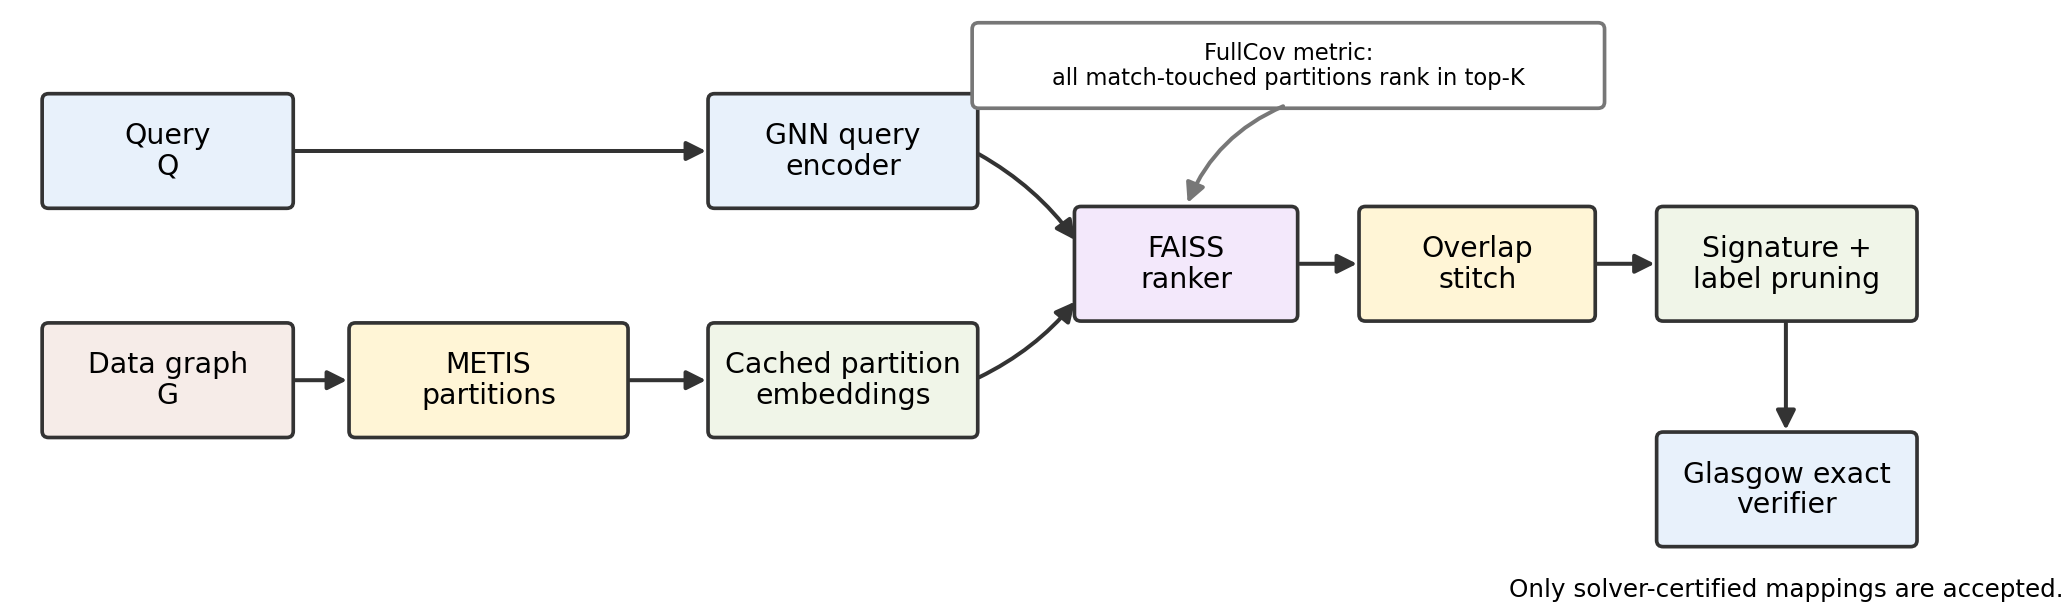
\includegraphics[width=\textwidth]{fig_jigsaw_pipeline.png}
\caption{\textbf{Jigsaw pipeline.} Offline work partitions and embeds the target. Online work embeds a query, retrieves coarse partitions, adds boundary overlap, prunes with query-derived invariants, and invokes Glasgow. Only Glasgow can accept a match.}
\label{fig:pipeline}
\end{figure}

Figure~\ref{fig:pipeline} gives the complete dataflow. \textbf{1. Prepare the target (offline).} METIS creates fine and coarse blocks. The shared encoder embeds every coarse block once, and FAISS indexes the normalized vectors. \textbf{2. Rank a query (online).} The same encoder maps a submitted query to $z_Q=f_\theta(Q)$ and retrieves the top-$K$ coarse blocks by cosine similarity. \textbf{3. Stitch boundaries.} For each retrieved block, Jigsaw adds only one-hop boundary nodes from adjacent blocks, not those blocks in full. \textbf{4. Prune and decompose.} Query-derived node-type, feature-signature, and exact-label tokens remove incompatible nodes; connected components become independent verifier calls. \textbf{5. Verify.} Glasgow searches the surviving components and is the only stage allowed to return a match.

As a running example, suppose a planted query touches blocks $p_4$ and $p_7$. If both rank in the top $K$, FullCov holds. If only $p_4$ ranks but the required nodes of $p_7$ lie on its boundary, overlap can still complete the candidate. Pruning then discards nodes whose invariant tokens do not occur in the query, and Glasgow either certifies a mapping or returns no match for that candidate. If an interior node of $p_7$ is never admitted, the bounded run may miss the match, but it cannot return an invalid one.

The shared encoder projects node features to 256 dimensions, applies six residual message-passing blocks with LayerNorm, pools global mean, max, and sum statistics, and emits a normalized 128-dimensional vector. Cora and Arxiv use GraphSAGE~\cite{ref_graphsage}; heterogeneous MAG retains node and relation types through a relational graph convolutional network (RGCN)~\cite{ref_rgcn}. Appendix~\ref{app:encoder} gives the full architecture.

\paragraph{FullCov objective.}
Standard contrastive training~\cite{ref_cpc} can leave one required partition ranked too low. We define the loss using the locked Arxiv configuration evaluated in Table~\ref{tab:loss_ablation}. For query $i$, let $P_i$ be its required partitions and $u_{ij}=z_i^\top p_j/\tau_{\mathrm{cov}}$. Each positive $j\in P_i$ receives
\begin{equation}
c_{ij}=-\log\frac{e^{u_{ij}}}{\sum_m e^{u_{im}}},\quad
h_i=\max_{n\notin P_i}u_{in},\quad
\ell_{ij}=c_{ij}+0.25\,\mathrm{softplus}(h_i-u_{ij}).
\end{equation}
For tail fraction $\rho$, $\mathrm{CVaR}_{\rho}$~\cite{ref_cvar} is the mean of the largest $\max(1,\lceil \rho|P_i|\rceil)$ losses, so easy positives cannot hide the weakest one. The top-$K$ barrier uses $t_i(K)$, the $(K-|P_i|+1)$-th largest negative score, and $b_{ij}=\mathrm{softplus}(t_i(K)-u_{ij})$. The implemented coverage loss is
\begin{equation}
\mathcal{L}_{\mathrm{cov}}=
\mathrm{CVaR}_{\rho}(\{\ell_{ij}\})+
0.35\,\mathrm{CVaR}_{\rho}(\{b_{ij}\}).
\end{equation}
For level $r\in\{\mathrm{fine},\mathrm{coarse}\}$, let $p_i^r$ be query $i$'s paired positive, $H_i^r$ its explicit hard negatives (empty at the fine level), and $s(a,b)=a^\top b$. The implemented in-batch term is
\begin{equation}
\mathcal{L}_{r\text{-NCE}}=-\frac{1}{B}\sum_i\log
\frac{e^{s(z_i,p_i^r)/0.1}}
{e^{s(z_i,p_i^r)/0.1}+\sum_{j\ne i}e^{s(z_i,p_j^r)/0.1}+\sum_{h\in H_i^r}e^{s(z_i,h)/0.1}}.
\end{equation}
When $|P_i|>K$, the effective budget increases to the next multiple of 10. The complete objective is $0.2\mathcal{L}_{\mathrm{fine\text{-}NCE}}+0.8\mathcal{L}_{\mathrm{coarse\text{-}NCE}}+\mathcal{L}_{\mathrm{cov}}$. Arxiv uses $K{=}20$, CVaR fraction $.25$, and up to 24 live required partitions. MAG uses the same form with $K{=}50$, CVaR fraction $.5$, and up to 64 live required partitions to reflect its larger true footprints. Cached partition embeddings keep both settings tractable while live positives update the query and partition paths.

\paragraph{Why the weakest positive.}
FullCov is a conjunction: every required partition must rank within $K$. The loss therefore emphasizes the worst positive rather than average similarity. Table~\ref{tab:loss_ablation} shows the largest gain at the fixed budgets used by the cascade. At inference, a positive can fail because retrieval and overlap miss the planted embedding or because Glasgow times out on a large candidate; the benchmark records both outcomes separately.

\section{Experimental Protocol}

\paragraph{Datasets.}
We evaluate Cora~\cite{ref_cora}, OGBN-Arxiv~\cite{ref_ogb}, and the full heterogeneous OGBN-MAG. Cora is small enough for exact timing sanity checks; Arxiv is the main medium-scale benchmark. OGBN-MAG contains 1{,}939{,}743 nodes of four types joined by typed relations. The MAG encoder retains those node and relation types through RGCN rather than collapsing the graph to attribute-only homogeneous structure.

\paragraph{Label granularity.}\label{sec:protocol} Glasgow matches discrete vertex labels, as in classical label-based graph indexing~\cite{ref_graphgrep,ref_gindex}. Our evaluation label semantics use $\sigma(v)=\mathrm{md5}(r(x_v))\bmod 10^{6}$, where $r$ records active indices for binary features and rounds dense feature values to four decimal places. The codebook is highly selective but not collision-free, so ``exact'' means exact graph matching under $\sigma$, not raw floating-point vector identity. A collision-free dictionary over distinct feature vectors, or a final raw-attribute equality guard, removes this distinction without changing retrieval or the soundness argument. At serving time, every label and signature token comes from the submitted query payload; planted target-node IDs remain evaluation metadata and never enter candidate construction. Selective labels make Cora and Arxiv \emph{label-rich}: once coverage is met, pruning collapses the candidate. Coarsened-label experiments weaken that signal and isolate the regime in which learned localization matters.

\paragraph{Queries and retrieval policies.}
The main benchmark uses two query seeds, three target sizes (20/50/100), and 50 queries per type/size/seed. Positive families are single-partition, multi-fine, K-hop, degree K-hop, random walk, and multi-coarse; negatives are negative-label and negative-structure. Every multi-region positive is a connected planted subgraph. Six policies isolate the main retrieval mechanisms: \textbf{Jigsaw} (learned GraphSAGE/RGCN partition ranker), \textbf{MeanFeat} (cosine on mean node features), \textbf{Mean-RRF} (reciprocal-rank fusion~\cite{ref_rrf} of the learned Jigsaw and MeanFeat rankings, which is a configuration of our own retriever rather than a nonparametric baseline), \textbf{TopoFeat} (coarse structural descriptors), \textbf{Random} (uninformed control), and \textbf{FilterAll} (all partitions to pruning/verification, serving as a recall ceiling rather than a scalable retriever). A seventh policy, \textbf{FeatureIndex}, is a classical label-coverage index in the GraphGrep~\cite{ref_graphgrep}/gIndex~\cite{ref_gindex} tradition that ranks partitions by how many of the query's exact labels they contain. We evaluate it on MAG to identify the label-selectivity crossover between classical and learned localization.

\paragraph{Partition and overlap scale.}
The partitions are balanced (MAG: 2{,}000 coarse partitions of median size 969, 10{,}000 fine partitions of median size 194). For a selected partition, the overlap operator adds only the \emph{boundary nodes} of partitions sharing an edge with it. This is a tight per-partition expansion ($5.4\times$ on MAG), far below the loose whole-neighbor-union bound it never realizes (Appendix~\ref{app:partitions}). Breadth arises only when the cascade unions these overlaps across the retrieval budget; the verifier sees the much smaller pruned candidate of Table~\ref{tab:production_matrix}. Appendix~\ref{app:partitions} (Tables~\ref{tab:partition_sizes},~\ref{tab:partition_overlap}) gives the full scale, and Section~\ref{sec:shrinkage} dissects how much each cascade stage removes.

\paragraph{Metrics.}
Retrieval uses partition recall@$K$ (required fraction retrieved) and FullCov@$K$ (all required retrieved). Positive solve rate counts planted queries verified within the time limit; negative no-match accuracy counts negatives completed without a mapping, with accepted negatives and timeouts reported separately. Candidate size is the terminal pruned node domain; cascade time accumulates candidate construction and verification across budgets. Each dataset has exactly 2,400 unique queries: 1,800 positives (6 families) and 600 negatives (2 families), from 2 seeds, 3 sizes, and 50 queries per cell. Across three datasets this is 7,200 unique queries, comprising 5,400 positives and 1,800 negatives. Applying 6 policies yields 14,400 policy-query evaluations per dataset before budget expansion; these are evaluation rows, not additional unique queries. As a dataset-integrity audit, the planted witnesses for all 1,800 MAG positives (101,951 node pairs), whether solved or not, agree in raw attributes, feature labels, and the serving-safe node-type/feature signature. Section~\ref{sec:soundness} separately audits 87,536 raw-equal query-to-target pairs supporting all 1,595 learned-Jigsaw acceptances. All 1,800 negatives use query-payload pruning. Diagnostic variants remain separate from the main grid.

\paragraph{Implementation, transfer, and reproducibility.} Partitioning uses METIS, partition vectors use FAISS, and exact verification uses Glasgow on integer-labelled candidates. A new query against an indexed target needs no retraining: it is embedded inductively and compared with cached partition vectors. For a new target graph, the partition hierarchy, partition embeddings, and FAISS index must be rebuilt. Encoder reuse across target graphs is not evaluated or claimed; each dataset or feature schema in our experiments uses its own trained encoder. Representative offline and online costs are reported in Appendix~\ref{app:encoder}. Per-query cascade timings use 8-vCPU Google Cloud instances and a $30$\,s verifier budget. We will release trained encoders, query seeds, partition hierarchies, and checksum-verified outputs. An anonymized implementation is available for review at \url{https://anonymous.4open.science/r/Jigsaw}.

\section{Results}

\subsection{FullCov Training Improves Retrieval}

Table~\ref{tab:loss_ablation} (visualized in Figure~\ref{fig:fullcov_ablation}) gives the controlled Arxiv retrieval comparison. All rows use the same locked K-hop query seeds, fixed retrieval budgets, and 9,000 optimizer steps. The FullCov objective improves the operating points most relevant to bounded exact verification.

\begin{table}[t]
\centering
\caption{\textbf{Controlled Arxiv retrieval-objective ablation.} Fixed retrieval budgets on $n{=}400$ locked K-hop queries (200 per query seed); each row averages the validation-selected checkpoint from two independent training replicates.}
\label{tab:loss_ablation}
\small
\setlength{\tabcolsep}{5pt}
\begin{tabular}{lcccc}
\toprule
\textbf{Objective} & \textbf{FullCov@20} & \textbf{FullCov@50} & \textbf{FullCov@100} & \textbf{Mean worst rank} \\
\midrule
Contrastive control & 21.7\% & 39.0\% & 66.0\% & 74.02 \\
FullCov objective & \textbf{26.0\%} & \textbf{48.8\%} & \textbf{82.0\%} & \textbf{58.97} \\
\midrule
McNemar $p$ & $4.6{\times}10^{-3}$ & $9.8{\times}10^{-6}$ & $4.0{\times}10^{-10}$ & -- \\
\bottomrule
\end{tabular}
\end{table}

The locked K-hop suite contains no queries that are impossible at $K=20,50,100$; the mean true coarse footprint is 6.37 and the maximum is 17. The remaining misses are ranking errors, and FullCov targets them by optimizing the weakest required partition. Both models use the same query seeds and training budget, ruling out easier queries or longer optimization as explanations for the gain. The largest improvement appears at FullCov@100, the cascade's operating point, where better ordering matters but the verifier still cannot search the whole graph.

\subsection{Three-Dataset Main Benchmark}
\label{sec:production}

Table~\ref{tab:production_matrix} reports the main benchmark metrics. Positive queries measure exact planted-match recovery; negative queries measure correct no-match behavior. The table also includes false positives, solver timeouts, average candidate nodes, cascade time, and verifier time. Cascade time sums candidate construction and exact verification; it excludes retrieval/ranking, whose index is built offline and whose implementation-specific latency is reported separately where measured. All values are reproducible from the released benchmark summaries.

\begin{table}[t]
\centering
\caption{\textbf{Main benchmark metrics.} Pos. uses the same half-partition budgets $K{=}10/100/1000$ (Cora/Arxiv/MAG); FilterAll uses the explicit all-partition ceiling. Neg. is audited no-match accuracy; FP counts negative false positives, while TO counts positive-query solver timeouts (FeatureIndex was run on positives only). Candidate and timing columns use the same endpoint as each Pos. entry. Cascade time is candidate construction plus exact verification and excludes retrieval/ranking.}
\label{tab:production_matrix}
\scriptsize
\setlength{\tabcolsep}{2.5pt}
\begin{tabular}{llrrrrrrr}
\toprule
\textbf{Dataset} & \textbf{Method} & \textbf{Pos. \%} & \textbf{Neg. \%} & \textbf{FP} & \textbf{TO} & \textbf{Cand. nodes} & \textbf{Cascade s} & \textbf{Solver ms} \\
\midrule
Cora & Jigsaw & 94.2 & 100.0 & 0 & 0 & 458 & 0.05 & 11.8 \\
Cora & Mean-RRF & 93.8 & 100.0 & 0 & 0 & 485 & 0.05 & 11.8 \\
Cora & MeanFeat & 87.7 & 100.0 & 0 & 0 & 1.13K & 0.06 & 10.5 \\
Cora & TopoFeat & 31.9 & 100.0 & 0 & 0 & 7.60K & 0.17 & 3.6 \\
Cora & Random & 32.7 & 100.0 & 0 & 0 & 7.54K & 0.16 & 3.8 \\
Cora & FilterAll$^\ddagger$ & 100.0 & 100.0 & 0 & 0 & 59 & 0.06 & 12.7 \\
\midrule
Arxiv & Jigsaw & 92.8 & 100.0 & 0 & 0 & 77 & 0.19 & 18.3 \\
Arxiv & Mean-RRF & 94.0 & 100.0 & 0 & 0 & 75 & 0.19 & 18.8 \\
Arxiv & MeanFeat & 89.7 & 100.0 & 0 & 0 & 91 & 0.22 & 18.4 \\
Arxiv & TopoFeat & 33.3 & 100.0 & 0 & 0 & 233 & 0.46 & 6.0 \\
Arxiv & Random & 39.2 & 100.0 & 0 & 0 & 219 & 0.47 & 7.0 \\
Arxiv & FilterAll$^\ddagger$ & 100.0 & 100.0 & 0 & 0 & 57 & 0.35 & 19.1 \\
\midrule
MAG & Jigsaw & \textbf{88.6} & 99.5 & 1 & 25 & 138.1K & 6.97 & 81.9 \\
MAG & Mean-RRF & 85.4 & 99.5 & 1 & 17 & 137.1K & 5.38 & 67.9 \\
MAG & FeatureIndex$^\S$ & \textbf{96.7} & -- & -- & 24 & 59.4K & 2.39 & 118.8 \\
MAG & MeanFeat & 64.6 & 99.5 & 1 & 12 & 212.1K & 8.02 & 27.5 \\
MAG & TopoFeat & 37.1 & 99.8 & 1 & 1 & 235.6K & 8.07 & 5.2 \\
MAG & Random & 51.4 & 99.7 & 1 & 9 & 282.1K & 9.54 & 19.9 \\
MAG & FilterAll$^\ddagger$ & 98.4 & 99.3 & 1 & 33 & 443.8K & 5.85 & 288.6 \\
\bottomrule
\end{tabular}
\end{table}

Cora and Arxiv reach $100\%$ only at the exhaustive all-partition budget (their 20/200 partitions), so those values are FilterAll ceilings rather than retrieval results. At the comparable half-partition budget, the overlap-aware GraphSAGE retriever solves $94.2\%$ on Cora and $92.8\%$ on Arxiv. Random and topology policies fall between $31.9\%$ and $39.2\%$ on Cora/Arxiv, and between $37\%$ and $51\%$ on MAG. Overlap-aware training lifts Arxiv from $74.1\%$ to $92.8\%$ at this budget, while Cora is already near saturation ($95.4\%\!\to\!94.2\%$). Mean-RRF is close at $93.8\%$/$94.0\%$, and a classical label index leads MAG under near-unique labels ($96.7\%$). Together, FullCov and the coarsened-label experiments identify the regime where learned localization contributes most.

MAG is the stress case: random and topology degrade sharply, mean features help, and the deployed MAG retriever reaches \textbf{88.6\%} while sending the verifier $3.2\times$ fewer candidate nodes than FilterAll (138K vs.\ 444K). Difficulty grows with query footprint rather than node count alone. Learned-Jigsaw recovery declines from $93.2\%$ at size 20 to $90.7\%$ at 50 and $82.0\%$ at 100, driven by random-walk queries, whose recovery falls from $94/100$ to $40/100$ as their planted footprint grows. Contained families are unaffected: multi-fine stays at $100/100$ and multi-coarse near three-quarters at every size. FilterAll reaches 98.4\%, but it gives the verifier all partitions and serves as a recall ceiling rather than a scalable policy. \textbf{The cascade never holds the whole graph resident:} it admits partitions one at a time and prunes with query-payload-derived structural-signature and exact-label sets before materializing edges. A conservative streaming serve (resident cache of eight partitions, survivor edges fetched in a second pass) peaks at \textbf{2.4\,GB} across a 54-query MAG grid (6 families $\times$ 3 sizes $\times$ 3 queries), compared with \textbf{10.2\,GB} to hold MAG for a direct solve. This is a $4.2\times$ reduction. The serve recovers $46/54$ planted matches (all easy-family queries; the 8 misses are random-walk/multi-coarse) and solves components with a median 110 nodes (maximum $9{,}497$) in 5\,ms to 8.4\,s.

\paragraph{Label-selectivity crossover.} Near-unique md5 labels give exact-label methods unusually strong signal. In that setting, the classical label-coverage index (\textbf{FeatureIndex}, GraphGrep/gIndex-style) is the strongest bounded retriever ($96.7\%$ solve, median worst-true-partition rank $104$ of $2{,}000$), ahead of the learned GNN ($88.6\%$; median rank ${\sim}900$). Once labels are coarsened, the localization ordering reverses. The learned ranker beats the label index in median worst-true-partition rank ($5$ vs.\ $7$ on Cora and $44$ vs.\ $104$ on Arxiv at class labels; Table~\ref{tab:selectivity_xd_log}) and leads in every MAG query family at coarse 39-class labels. Complete coarse-label solve runs are statistically tied (FeatureIndex $63.4\%$; learned variants between $63\%$ and $64\%$). The validated learning result is therefore localization: the GNN becomes the better partition ranker after exact labels lose selectivity. Sweeping the MAG codebook itself from near-unique to near-degenerate labels reproduces the same crossover on one target (Appendix~\ref{app:probes}, Table~\ref{tab:mag_selectivity_sweep}).

The same transition breaks resident exact pipelines. With MAG labels coarsened to 32 deterministic buckets, CFL-Match, DP-iso, and GQL complete only $12/27$ solver-query executions: $8/9$ at size 20 but $2/9$ at each of sizes 50 and 100, with random-walk worst at $3/9$. Candidate tables reach $2.4$M entries and 15 calls hit the 120\,s limit. The monotone size effect locates the failure in whole-graph candidate construction as label selectivity falls. Under the original selective labels, the same matchers finish all $27/27$ executions once the graph is resident.

Spatial footprint explains the remaining retrieval gap. The learned ranker localizes contained queries almost perfectly (single/multi-fine ranks from $3$ to $7$), while diffuse families require coverage across many distant partitions. The inference-time variants in Appendix~\ref{app:probes} leave FullCov@1000 within ${\approx}2$ points, locating the bottleneck in the single-vector representation rather than score aggregation. An offline label-selectivity statistic chooses between the label index and learned ranker without changing the downstream cascade. Within the learned policy, FullCov and aligned training improve random-walk and multi-coarse coverage and lift Arxiv from $74.1\%$ to $92.8\%$. The systems result is memory-bounded exact verification, and the learning result is improved coverage where label indexing no longer localizes reliably.

Direct Glasgow provides the CP-verifier control. Full-graph matching with no retrieval solves \textbf{0 of 15} sampled MAG K-hop queries, with no query returning before the timeout. Under this resource budget, retrieval is necessary for Glasgow rather than a minor optimization. The same configuration solves all 15 Cora queries but \textbf{0 of 15} on OGBN-Arxiv (169K nodes), while Jigsaw remains feasible by handing Glasgow a $\sim\!50$-node pruned candidate (Table~\ref{tab:scaling_latency}, Figure~\ref{fig:scaling}). This places the tested crossover between Cora and Arxiv. Resident filter-and-verify matchers can be faster after loading when labels are selective; Section~\ref{sec:limits} scopes our claim to Glasgow, bounded-memory service, and the low-selectivity regime. Mean-RRF (85.4\%) fuses the learned and mean-feature rankings within Jigsaw, and the pure learned ranker leads it by $3.2$ points. Both exceed the mean-feature baseline ($64.6\%$) by more than 20 points. These configurations occupy different points on the same recall-cost frontier (Appendix~\ref{app:mag_narrative}).

\begin{figure}[tb]
\centering
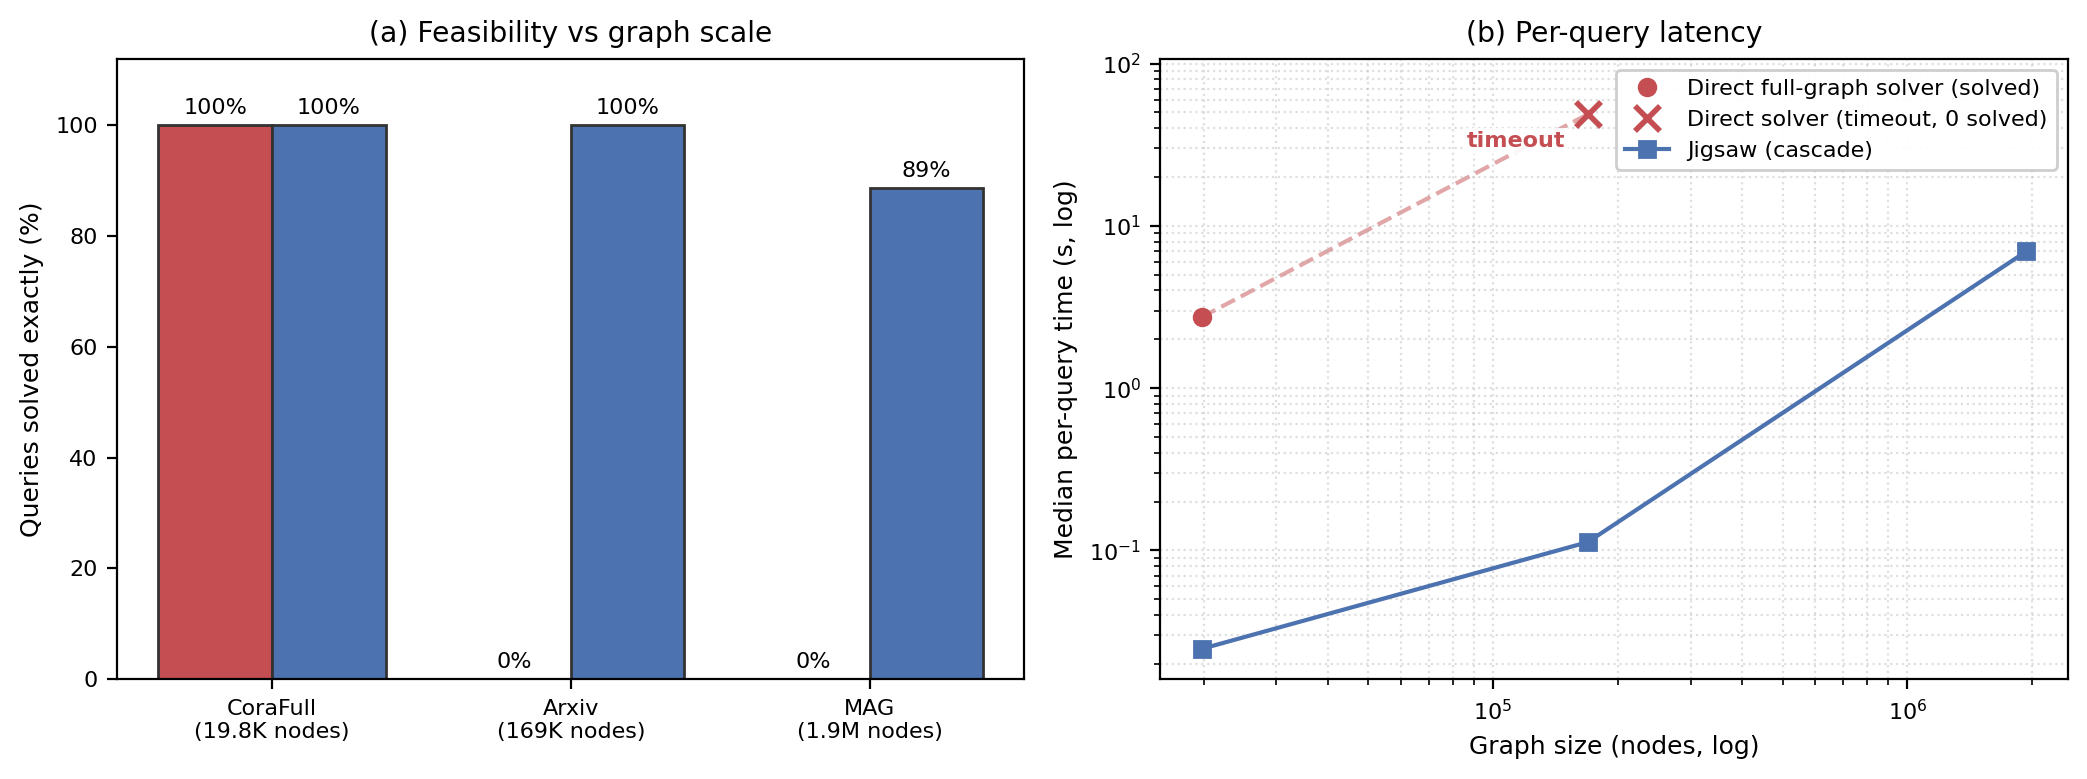
\includegraphics[width=0.82\textwidth]{fig_scaling_feasibility.png}
\caption{\textbf{Jigsaw makes the exact solver's domain tractable.} Cora/Arxiv use the same 15 K-hop queries at equal half-partition budgets ($K=10/100$), where Jigsaw solves 15/15 on both; the MAG cascade point is the separate 1,800-positive main-benchmark mean at $K=1{,}000$. Direct Arxiv is timeout-censored in the latency panel; the MAG control records the 0/15 timeout outcome but no comparable wall-clock point.}
\label{fig:scaling}
\end{figure}

\begin{table}[t]
\centering
\caption{\textbf{Scaling and latency: direct full-graph solver vs.\ Jigsaw cascade.} Cora/Arxiv use the same 15 K-hop queries and Jigsaw is evaluated at equal half-partition budgets ($K=10/100$), avoiding exhaustive Cora retrieval. The MAG direct cell uses its 15-query timeout control, while $^\ast$ the MAG Jigsaw cell is separately the 1,800-positive main-benchmark mean at $K=1{,}000$. $^\dagger$ Glasgow's 30\,s Arxiv budget may be exceeded during cleanup/loading.}
\label{tab:scaling_latency}
\small
\begin{tabular}{l r c r c r r}
\toprule
 & & \multicolumn{2}{c}{Direct full-graph solver} & \multicolumn{2}{c}{Jigsaw cascade} & Cand.\ \\
\cmidrule(lr){3-4}\cmidrule(lr){5-6}
Dataset & Nodes & Solved & Med.\ time & Solved & Med.\ time & nodes \\
\midrule
Cora  & 19.8K & 15/15 & $2.74$\,s & 15/15 & $\mathbf{0.03}$\,s & 50 \\
Arxiv & 169K  & \textbf{0/15}$^\dagger$ & ${\approx}49$\,s & 15/15 & $\mathbf{0.11}$\,s & 50 \\
MAG   & 1.9M  & \textbf{0/15} & timeout & 88.6\% & $6.97$\,s$^\ast$ & -- \\
\bottomrule
\end{tabular}
\end{table}

Bootstrap 95\% confidence intervals and paired exact-McNemar tests on the MAG solve rate confirm this ordering among the interchangeable retrieval \emph{components} (full statistics, per-family solve rates, and budget curves in Appendices~\ref{app:mag_narrative} and~\ref{app:family}). These comparisons evaluate retrieval components within the same surrounding system. That system enables exact matching at scale without holding the graph resident, while FullCov secures coverage on the hard families.

\subsection{Candidate-Shrinkage Cascade and Boundary Overlap}
\label{sec:shrinkage}

All reported main-benchmark solve rates use one-hop boundary overlap: selected partitions admit boundary nodes from adjacent partitions, not the neighboring partitions in full. To test whether unioning this boundary overlap makes partitioning irrelevant, we measure the per-query cascade $\text{full graph} \to \text{overlap} \to \text{signature} \to \text{label-pruned} \to \text{solver}$ on 14{,}400 positive method/model-query evaluation records over the 1{,}800-query MAG positive grid from a separately controlled shrinkage run at the decided budget. Hybrid and Mean-RRF each contribute two model variants, so 14{,}400 is an evaluation-record count rather than a unique-query denominator. Three facts emerge. \textbf{(1) The union is broad, but ranking still removes most of the graph:} the median overlap union is 59\% of MAG for Jigsaw, compared with 73\% to 83\% for mean-feature, random, and topology retrieval. After identical pruning, Jigsaw's median candidate has 84.5K nodes versus 544K for FilterAll (Table~\ref{tab:production_matrix} reports means, 138.1K vs.\ 443.8K). Ranking alone accounts for this $6.4\times$ reduction.

\textbf{(2) All planted-node coverage loss occurs by the overlap stage; pruning is coverage-lossless.} This follows from the pruning operator, not only from the measurements.

\begin{proposition}[Lossless pruning]
\label{prop:lossless}
Let the pruning token $\sigma(\cdot)$ be a node attribute that the matching semantics preserve, i.e.\ any valid embedding $\phi$ of $Q$ into $G$ satisfies $\sigma(\phi(q))=\sigma(q)$ for every query node $q$ (vertex-labelled matching, with $\sigma$ derived from node type and feature labels). Prune the candidate $G_C$ to $G_C'=\{v\in G_C : \sigma(v)\in \sigma(V_Q)\}$. Then for any embedding $\phi$ with $\phi(V_Q)\subseteq G_C$, we have $\phi(V_Q)\subseteq G_C'$. Hence pruning preserves node coverage: $\mathrm{FullCov}$ is unchanged.
\end{proposition}
\noindent\emph{Proof.} For $q\in V_Q$, $\sigma(\phi(q))=\sigma(q)\in\sigma(V_Q)$, so $\phi(q)$ satisfies the keep condition and is retained. Thus every matched node survives.

The cascade signatures (node type $\times$ feature-bit hashes) and the exact label filter are such attribute invariants, so Proposition~\ref{prop:lossless} applies; a \emph{degree}-based token would not be matching-invariant ($\deg(\phi(q))\ge\deg(q)$ only), which is why the pipeline prunes on attributes, not degree. Empirically, for every policy the planted-match survival rate after overlap equals that after pruning (Jigsaw $87\%$ both in the same controlled shrinkage run, whose end-to-end solve rate is $86.0\%$). Candidate coverage therefore sets the dominant solve ceiling; the remaining gap is recorded separately as verifier timeouts.

\textbf{(3) Latency is dominated by candidate construction, not solving} (per-query build $\gg$ solve; Appendix~\ref{app:mag_narrative}): the verifier is cheap, and assembling the broad overlap union is the cost.

\paragraph{Boundary overlap is an essential recall operator.}
The matched operator ablation shows its effect directly: removing boundary overlap cuts MAG solve rate from $88.9\%$ to $44.4\%$ and Arxiv from $94.4\%$ to $86.1\%$ (Appendix~\ref{app:design}). Its benefit is strongest for compact local structure. When retrieval misses a true partition, one-hop boundary overlap recovers it for $94\%$ of K-hop queries but for $62\%$ of random-walk queries, whose matches more often extend into the interior of an unselected partition. This family dependence explains why overlap sharply raises overall recovery while diffuse random-walk queries remain the hardest case. Together with the lossless-pruning result above, the measurements locate every coverage loss before verification: whenever the planted match survives retrieval plus overlap, pruning retains it. Verifier timeouts remain a separate reported outcome.

\subsection{Negative Queries and Soundness}
\label{sec:soundness}

Jigsaw only accepts after Glasgow verification, so the negative families test no-match behavior under the configured labels. Accuracy is $100.0\%$ on Cora/Arxiv and $99.3\%$ to $99.8\%$ across MAG policies. We audited every learned-Jigsaw MAG positive acceptance before hashing. Of 1,595 acceptances, 1,513 candidates retain the planted bitwise-equal witness (83,656 query-to-target pairs). Replaying the remaining 82 at their exact accepted budget and candidate under query-payload pruning solves all 82; all 3,880 returned pairs are bitwise equal. The full audit covers 87,536 accepted positive pairs with zero raw mismatches. Among 600 MAG negatives, FilterAll accepts one structure-perturbed query, also flagged by every policy. Its exhaustive replay returns one 20-node mapping, and all 20 pairs are bitwise equal. No learned-Jigsaw MAG positive acceptance, nor the sole FilterAll MAG negative acceptance, depends on a hash collision. Directly measuring the codebook, hashing the $736{,}389$ featured MAG paper nodes gives $521{,}393$ occupied codes, with $168{,}258$ buckets holding at least two distinct canonicalized feature vectors, so $52.0\%$ of featured nodes fall in a $\sigma$-colliding bucket ($29.2\%$ excess), consistent with uniform hashing into $10^6$ buckets. The latter acceptance shows that this synthetic negative is not a valid global non-existence certificate: an alternative raw-attribute-preserving embedding exists. Bounded no-match results remain candidate-local, while completed FilterAll verification is globally complete under $\sigma$.

\section{Discussion and Limitations}
\label{sec:limits}

Jigsaw preserves exact verification while using learned retrieval to choose the search boundary. If retrieval misses a required region, the solver cannot recover that match; FullCov turns this source of incompleteness into a measurable training and serving objective. The design targets static graphs with repeated queries, where partitioning, embedding, and FAISS indexing amortize. Cora and Arxiv expose saturation under selective labels, while MAG separates the policies: FeatureIndex leads with near-unique labels while learned retrieval localizes better after labels are coarsened. FilterAll remains the exhaustive upper bound against which bounded retrieval is measured. All three evaluated targets are citation graphs; the pipeline makes no citation-specific assumption---METIS, FAISS, typed-signature pruning, and Glasgow apply to any typed attributed graph---so transfer to other topologies (social, molecular, spatial, road) is an open empirical question rather than an architectural limit, and our primary future direction.

\paragraph{Evaluation scope.} We compare against classical feature/structure-index rankers (MeanFeat/TopoFeat, GraphGrep~\cite{ref_graphgrep}/gIndex~\cite{ref_gindex}-style filters), a no-retrieval exact control (full-graph Glasgow, $0/15$ MAG), an exhaustive FilterAll upper bound, and uninformed retrievers. We also benchmark scalable filter-and-verify matchers (CFL-Match, DP-iso, GQL): they solve Cora/Arxiv and high-selectivity MAG once loaded, while completing only $12/27$ coarse-label MAG solver-query executions. Together these controls locate Jigsaw's advantage in the CP-based Glasgow path, bounded-memory service, and low-selectivity candidate construction. NeuroMatch and GLSearch use released protocols for smaller, contained-query targets rather than a partitioned million-node execution path. Out-of-core and distributed systems (DUALSIM~\cite{ref_dualsim}, STwig/Trinity~\cite{ref_trinity}, G-thinker~\cite{ref_gthinker}) address residence by streaming or sharding the entire graph; Jigsaw instead uses learned region relevance to expose a tunable single-machine memory frontier. Its one-time target preparation and training costs amortize over repeated queries; Appendix~\ref{app:encoder} reports the measured hierarchy-load, embedding, indexing, training, and query-ranking costs. The negative families are audited synthetic no-match tests, and the positives are planted connected subgraphs on static graphs. We therefore report no-match accuracy rather than global negative completeness and separate bounded retrieval from the FilterAll ceiling. Within this scope, FullCov improves hard-family coverage and the complete cascade turns the tested Glasgow operating point from $0/15$ direct solves into $88.6\%$ exact positive recovery.

The GNN-PE public-release diagnostic is reported in Appendix~\ref{app:gnnpe}.

\section{Conclusion}

Jigsaw turns learned graph retrieval into an execution mechanism for exact search. The model decides which regions deserve memory; Glasgow alone accepts a match. On full MAG, this changes the tested operating point from 0/15 direct CP solves to 88.6\% exact positive recovery, while streaming at 2.4\,GB instead of 10.2\,GB for whole-graph residence. FullCov trains against the system's decisive failure event: missing even one required partition. Boundary overlap recovers cross-partition matches, and lossless query-derived pruning bounds the verifier domain. Two operating regimes appear in the data: selective labels favor resident exact methods because their candidate tables collapse, while weak labels and bounded residency make whole-graph candidate construction fail. Jigsaw stays feasible in the latter regime through an adaptive portfolio---classical indexing when exact labels localize well, learned ranking when they do not, with FullCov improving the hard families. Jigsaw makes exact verification usable on million-node static graphs under a measurable memory budget without replacing exactness with a neural guess.

% ============================ APPENDIX ============================

{\small
\setlength{\bibsep}{0pt}
\begin{thebibliography}{42}

\bibitem[McCreesh et al.(2020)]{ref_glasgow}
McCreesh, C., Prosser, P., Trimble, J.: The Glasgow Subgraph Solver: Using Constraint Programming to Tackle Hard Subgraph Isomorphism Problem Variants. In: CP 2020, LNCS, vol. 12333, pp. 316--333. Springer (2020)

\bibitem[Xu et al.(2019)]{ref_gin}
Xu, K., Hu, W., Leskovec, J., Jegelka, S.: How Powerful are Graph Neural Networks? In: ICLR (2019)

\bibitem[Hamilton et al.(2017)]{ref_graphsage}
Hamilton, W.L., Ying, R., Leskovec, J.: Inductive Representation Learning on Large Graphs. In: NeurIPS, pp. 1024--1034 (2017)

\bibitem[Schlichtkrull et al.(2018)]{ref_rgcn}
Schlichtkrull, M., Kipf, T.N., Bloem, P., van den Berg, R., Titov, I., Welling, M.: Modeling Relational Data with Graph Convolutional Networks. In: ESWC, pp. 593--607 (2018)

\bibitem[Cordella et al.(2004)]{ref_vf2}
Cordella, L.P., Foggia, P., Sansone, C., Vento, M.: A (Sub)Graph Isomorphism Algorithm for Matching Large Graphs. IEEE TPAMI \textbf{26}(10), 1367--1372 (2004)

\bibitem[Johnson et al.(2021)]{ref_faiss}
Johnson, J., Douze, M., J\'egou, H.: Billion-Scale Similarity Search with GPUs. IEEE Trans. Big Data \textbf{7}(2), 535--547 (2021)

\bibitem[Karypis and Kumar(1998)]{ref_metis}
Karypis, G., Kumar, V.: A Fast and High Quality Multilevel Scheme for Partitioning Irregular Graphs. SIAM J. Sci. Comput. \textbf{20}(1), 359--392 (1998)

\bibitem[Hu et al.(2020)]{ref_ogb}
Hu, W., et al.: Open Graph Benchmark: Datasets for Machine Learning on Graphs. In: NeurIPS (2020)

\bibitem[Garey and Johnson(1979)]{ref_garey}
Garey, M.R., Johnson, D.S.: Computers and Intractability: A Guide to the Theory of NP-Completeness. W.H. Freeman (1979)

\bibitem[Ullmann(1976)]{ref_ullmann}
Ullmann, J.R.: An Algorithm for Subgraph Isomorphism. J. ACM \textbf{23}(1), 31--42 (1976)

\bibitem[Bonnici et al.(2013)]{ref_ri}
Bonnici, V., Giugno, R., Pulvirenti, A., Shasha, D., Ferro, A.: A Subgraph Isomorphism Algorithm and Its Application to Biochemical Data. BMC Bioinformatics \textbf{14}(Suppl 7), S13 (2013)

\bibitem[Solnon(2010)]{ref_lad}
Solnon, C.: AllDifferent-Based Filtering for Subgraph Isomorphism. Artificial Intelligence \textbf{174}(12--13), 850--864 (2010)

\bibitem[Sen et al.(2008)]{ref_cora}
Sen, P., Namata, G., Bilgic, M., Getoor, L., Galligher, B., Eliassi-Rad, T.: Collective Classification in Network Data. AI Magazine \textbf{29}(3), 93--106 (2008)

\bibitem[Ying et al.(2020)]{ref_neuromatch}
Ying, R., et al.: Neural Subgraph Matching. arXiv:2007.03092 (2020)

\bibitem[Ye et al.(2024)]{ref_gnnpe}
Ye, Y., Lian, X., Chen, M.: Efficient Exact Subgraph Matching via GNN-based Path Dominance Embedding. Proc. VLDB Endow. \textbf{17}(7), 1628--1641 (2024)

\bibitem[Liu et al.(2021)]{ref_glsearch}
Liu, Y., et al.: GLSearch: Maximum Common Subgraph Detection via Learning to Search. In: ICML (2021)

\bibitem[Liu et al.(2020)]{ref_nsic}
Liu, X., Pan, H., He, M., Song, Y., Jiang, X., Shang, L.: Neural Subgraph Isomorphism Counting. In: KDD (2020)

\bibitem[Han et al.(2013)]{ref_turboiso}
Han, W.S., Lee, J., Lee, J.H.: TurboISO: Towards Ultrafast and Robust Subgraph Isomorphism Search in Large Graph Databases. In: SIGMOD, pp. 337--348 (2013)

\bibitem[Bi et al.(2016)]{ref_cflmatch}
Bi, F., Chang, L., Lin, X., Qin, L., Zhang, W.: Efficient Subgraph Matching by Postponing Cartesian Products. In: SIGMOD, pp. 1199--1214 (2016)

\bibitem[Han et al.(2019)]{ref_daf}
Han, M., Kim, H., Gu, G., Park, K., Han, W.S.: Efficient Subgraph Matching: Harmonizing Dynamic Programming, Adaptive Matching Order, and Failing Set Together. In: SIGMOD, pp. 1429--1446 (2019)

\bibitem[He and Singh(2008)]{ref_graphql}
He, H., Singh, A.K.: Graphs-at-a-Time: Query Language and Access Methods for Graph Databases. In: SIGMOD, pp. 405--418 (2008)

\bibitem[Carletti et al.(2018)]{ref_vf3}
Carletti, V., Foggia, P., Saggese, A., Vento, M.: Challenging the Time Complexity of Exact Subgraph Isomorphism for Huge and Dense Graphs with VF3. IEEE Trans. Pattern Anal. Mach. Intell. \textbf{40}(4), 804--818 (2018)

\bibitem[Zeng et al.(2020)]{ref_gsi}
Zeng, L., Zou, L., \"{O}zsu, M.T., Hu, L., Zhang, F.: GSI: GPU-friendly Subgraph Isomorphism. In: ICDE, pp. 1249--1260 (2020)

\bibitem[Sun and Luo(2020)]{ref_survey}
Sun, S., Luo, Q.: In-Memory Subgraph Matching: An In-depth Study. In: SIGMOD, pp. 1083--1098 (2020)

\bibitem[Zhang et al.(2024)]{ref_survey2024}
Zhang, Z., Lu, Y., Zheng, W., Lin, X.: A Comprehensive Survey and Experimental Study of Subgraph Matching: Trends, Unbiasedness, and Interaction. Proc. ACM Manag. Data \textbf{2}(1), Article 60 (2024)

\bibitem[Mhedhbi and Salihoglu(2019)]{ref_wcoj}
Mhedhbi, A., Salihoglu, S.: Optimizing Subgraph Queries by Combining Binary and Worst-Case Optimal Joins. Proc. VLDB Endow. \textbf{12}(11), 1692--1704 (2019)

\bibitem[Ammar et al.(2018)]{ref_lowmem}
Ammar, K., McSherry, F., Salihoglu, S., Joglekar, M.: Distributed Evaluation of Subgraph Queries Using Worst-Case Optimal Low-Memory Dataflows. Proc. VLDB Endow. \textbf{11}(6), 691--704 (2018)

\bibitem[Kim et al.(2016)]{ref_dualsim}
Kim, H., Lee, J., Bhowmick, S.S., Han, W.-S., Lee, J., Ko, S., Jarrah, M.H.A.: DUALSIM: Parallel Subgraph Enumeration in a Massive Graph on a Single Machine. In: SIGMOD, pp. 1231--1245 (2016)

\bibitem[Sun et al.(2012)]{ref_trinity}
Sun, Z., Wang, H., Wang, H., Shao, B., Li, J.: Efficient Subgraph Matching on Billion Node Graphs. Proc. VLDB Endow. \textbf{5}(9), 788--799 (2012)

\bibitem[Yan et al.(2020)]{ref_gthinker}
Yan, D., Guo, G., Chowdhury, M.M.R., \"{O}zsu, M.T., Ku, W.-S., Lui, J.C.S.: G-thinker: A Distributed Framework for Finding Qualified Subgraphs in a Big Graph with Load Balancing. In: ICDE (2020)

\bibitem[Bai et al.(2019)]{ref_simgnn}
Bai, Y., Ding, H., Bian, S., Chen, T., Sun, Y., Wang, W.: SimGNN: A Neural Network Approach to Fast Graph Similarity Computation. In: WSDM, pp. 384--392 (2019)

\bibitem[Li et al.(2019)]{ref_gmn}
Li, Y., Gu, C., Dullien, T., Vinyals, O., Kohli, P.: Graph Matching Networks for Learning the Similarity of Graph Structured Objects. In: ICML, PMLR \textbf{97}, 3835--3845 (2019)

\bibitem[Xu et al.(2021)]{ref_psimgnn}
Xu, H., Duan, Z., Wang, Y., Feng, J., Chen, R., Zhang, Q., Xu, Z.: Graph Partitioning and Graph Neural Network Based Hierarchical Graph Matching for Graph Similarity Computation. Neurocomputing \textbf{439}, 348--362 (2021)

\bibitem[Roy et al.(2022)]{ref_isonet}
Roy, I., Velugoti, V.S.B.R., Chakrabarti, S., De, A.: Interpretable Neural Subgraph Matching for Graph Retrieval. In: AAAI \textbf{36}(7), 8115--8123 (2022)

\bibitem[Ramachandran et al.(2024)]{ref_isonetpp}
Ramachandran, A., Raj, V., Roy, I., Chakrabarti, S., De, A.: Iteratively Refined Early Interaction Alignment for Subgraph Matching Based Graph Retrieval. In: NeurIPS \textbf{37} (2024)

\bibitem[Raj et al.(2025)]{ref_neuraldesign}
Raj, V., Roy, I., Ramachandran, A., Chakrabarti, S., De, A.: Charting the Design Space of Neural Graph Representations for Subgraph Matching. In: ICLR (2025)

\bibitem[Ying et al.(2026)]{ref_neugn}
Ying, Y., Dai, Y., Li, W., et al.: Neural Graph Navigation for Intelligent Subgraph Matching. In: AAAI \textbf{40}(19), 16181--16189 (2026)

\bibitem[Shasha et al.(2002)]{ref_graphgrep}
Shasha, D., Wang, J.T.L., Giugno, R.: Algorithmics and Applications of Tree and Graph Searching. In: PODS, pp. 39--52 (2002)

\bibitem[Yan et al.(2004)]{ref_gindex}
Yan, X., Yu, P.S., Han, J.: Graph Indexing: A Frequent Structure-based Approach. In: SIGMOD, pp. 335--346 (2004)

\bibitem[van den Oord et al.(2018)]{ref_cpc}
van den Oord, A., Li, Y., Vinyals, O.: Representation Learning with Contrastive Predictive Coding. arXiv:1807.03748 (2018)

\bibitem[Rockafellar and Uryasev(2000)]{ref_cvar}
Rockafellar, R.T., Uryasev, S.: Optimization of Conditional Value-at-Risk. Journal of Risk \textbf{2}(3), 21--41 (2000)

\bibitem[Cormack et al.(2009)]{ref_rrf}
Cormack, G.V., Clarke, C.L.A., Buettcher, S.: Reciprocal Rank Fusion Outperforms Condorcet and Individual Rank Learning Methods. In: SIGIR, pp. 758--759 (2009)

\end{thebibliography}
}

\clearpage
\appendix
\raggedbottom

%% ===================================================================
%% Appendix order: Method (A-B) -> Results (C-D) -> Ablations/Analysis
%% (E-F) -> Memory (G). Figures live in the section they support.
%% ===================================================================

\section{GNN-PE Public-Release Diagnostic}
\label{app:gnnpe}

Beyond the internal policies, our external baselines include the direct-solver control (Table~\ref{tab:scaling_latency}, $0/15$ on Arxiv/MAG) and a GNN-PE public-release diagnostic. On Cora the released pipeline passes its self-test but, after class-label export and build repairs, recovers $7/24$ planted positives at $e=4$ (6 diagnostic families $\times$ 4 sizes $\times$ 1 query; $0/6$ at size 100). The release exposes an inference path but no supervised training recipe for this protocol, so the result measures public-release transfer rather than a retrained reproduction.

\section{Encoder Architecture and Training Interface}
\label{app:encoder}

\begin{figure}[h]
\centering
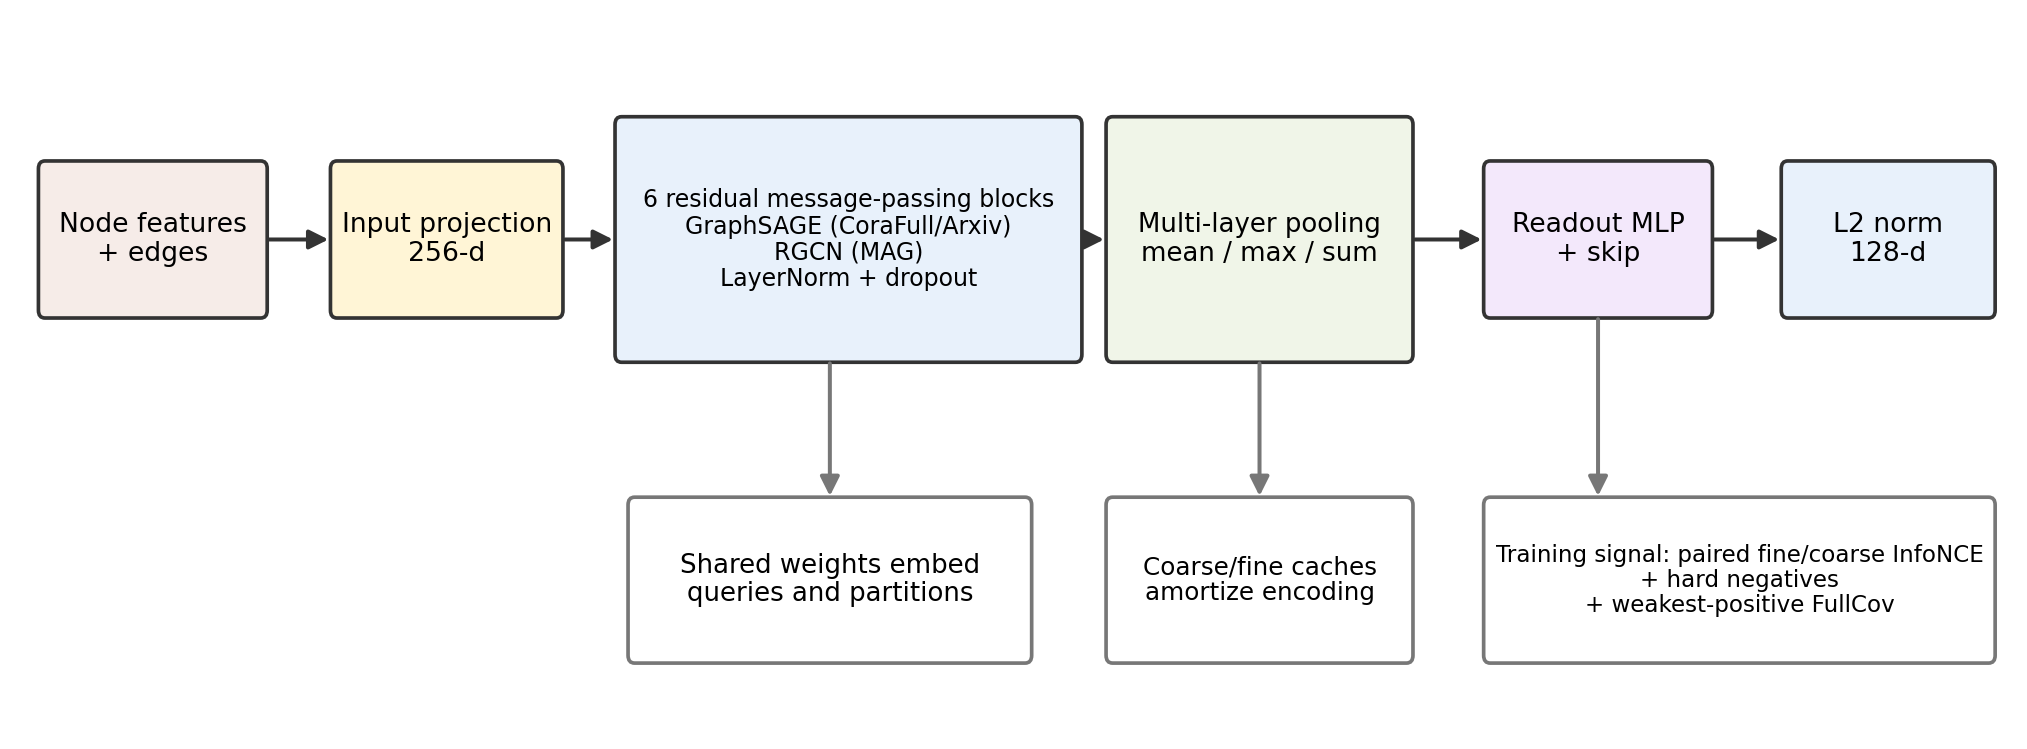
\includegraphics[width=\textwidth]{fig_encoder_architecture.png}
\caption{\textbf{Retrieval encoder.} Cora and Arxiv use a six-block residual GraphSAGE encoder; MAG uses the same six-block residual architecture with relation-aware RGCN layers. The same encoder embeds queries and cached graph partitions into a normalized 128-dimensional space.}
\label{fig:encoder}
\end{figure}

The encoder is intentionally shared between query graphs and partition graphs. Input node features are projected to a 256-dimensional hidden space, passed through six residual message-passing blocks, normalized with LayerNorm, and read out with multi-layer global mean, max, and sum pooling. The readout is an MLP plus a skip projection, followed by L2 normalization to produce a 128-dimensional retrieval vector. This matters because the retrieval problem is not node alignment; it is region localization. The model must place a query near every partition needed for exact verification, including the weakest or farthest true partition.

For Cora and Arxiv, the message-passing block is GraphSAGE~\cite{ref_graphsage} ($\mathtt{SAGEConv}$); on these label-rich graphs a matched objective ablation finds GraphSAGE at least as strong as a GIN encoder at the fixed budgets the cascade uses, so we adopt it as the homogeneous-graph encoder. OGBN-MAG is a \emph{heterogeneous} academic graph (paper, author, institution, and field-of-study nodes joined by typed relations); we flatten it to a single node/edge index for the pipeline but \emph{retain} node types and relation (edge) types and model them with a relation-aware six-layer RGCN~\cite{ref_rgcn} ($\mathtt{RGCNConv}$ with per-relation bases over $2R$ relations after symmetrization). Because OGBN-MAG supplies input features only on paper nodes, non-paper nodes receive node-type one-hot and per-relation-degree features, so the retriever reasons over typed structure rather than discarding it. Both encoders use the same retrieval interface: cached fine and coarse partition embeddings are compared to query embeddings, and positive partitions can be live-reencoded during training so coverage gradients update required positives instead of treating the entire partition bank as stale constants.

Training uses three complementary signals: paired fine/coarse InfoNCE aligns each query with sampled positive partitions; hard negatives keep nearby but incorrect partitions separated; and the FullCov term covers every coarse partition touched by the planted match while penalizing the weakest required positive. For MAG, the deployed checkpoint is selected by validation FullCov rather than by training epoch; the final-epoch checkpoint is retained only as a separate model diagnostic and is never averaged into the main benchmark.

\paragraph{Deployment boundary and measured setup costs.}
Queries are inductive with respect to an already indexed target: they use the shared encoder and require no fine-tuning. Target transfer is different. For a new graph, Jigsaw constructs and stores a METIS hierarchy, embeds its coarse partitions, and builds a FAISS index. The current paper does not claim zero-shot accuracy across datasets; each reported dataset has its own trained encoder. Table~\ref{tab:deployment_costs} separates target setup and training from online ranking; embedding and FAISS construction are one combined measurement. A retained MAG construction sweep built three independent hierarchies of approximately 2,000 coarse partitions in 57.4 minutes, or 19.1 minutes per hierarchy on average; the hierarchy is then reused across training and serving.

\begin{table}[h]
\centering
\caption{\textbf{Representative deployment costs.} Hierarchy loading and combined embedding-plus-index construction are measured setup runs; training is a one-time dataset cost; rank time is query encoding plus FAISS search and excludes candidate construction.}
\label{tab:deployment_costs}
\small
\setlength{\tabcolsep}{6pt}
\begin{tabular}{lrrrr}
\toprule
Target & Hierarchy load & Embed + index & Encoder training & Rank/query \\
\midrule
Arxiv (200 coarse) & 3.5\,s & 1.9\,s & 2--3\,h (9,000 steps) & 5.1\,ms \\
MAG (2,000 coarse) & 110.9\,s & 13.7\,s & ${\sim}3$\,h (5,000 steps) & 21.9\,ms \\
\bottomrule
\end{tabular}
\end{table}

\begin{figure}[h]
\centering
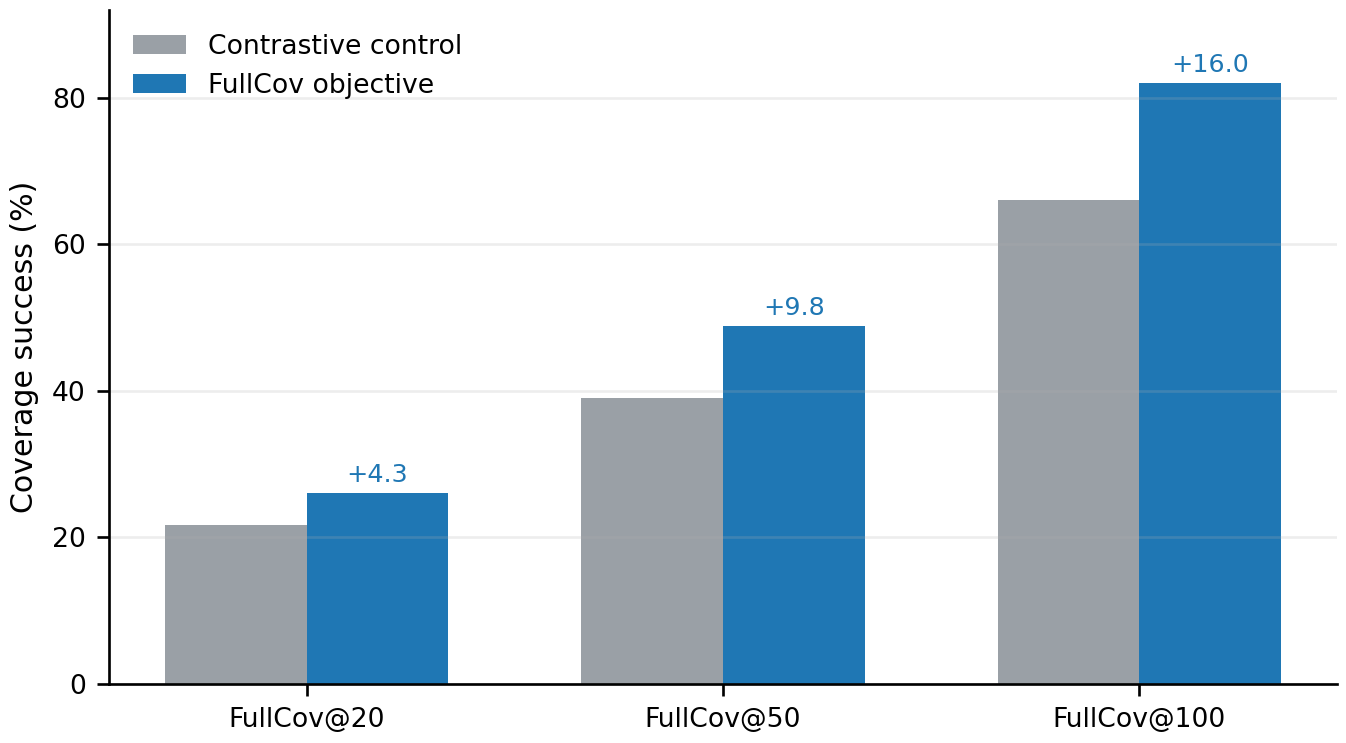
\includegraphics[width=0.85\textwidth]{fig_fullcov_ablation.png}
\caption{\textbf{FullCov objective gain.} Under matched Arxiv K-hop training conditions, directly optimizing weakest-positive coverage improves every fixed retrieval budget used by the downstream cascade.}
\label{fig:fullcov_ablation}
\end{figure}

\section{Partition Balance and Overlap Scale}
\label{app:partitions}

The experiments use the hierarchy below. For a selected partition $p$, the overlap operator adds only boundary nodes from other partitions that share an edge with $p$, rather than adding the entire bordering partitions. On MAG, a median partition borders 948 of the 2{,}000 coarse partitions, but it admits only about 4{,}252 boundary nodes. The expanded region for one selected partition is therefore about 5{,}228 nodes (a $5.4\times$ expansion over the 969-node partition), not the $\approx$921K obtained by taking every bordering partition in full. That 921K figure is a loose reachability bound the operator never realizes. Candidate size grows only when the cascade unions boundary overlap from hundreds to a thousand retrieved partitions. Because many boundary nodes are shared, the union saturates between 59\% and 83\% of MAG at the largest budgets (59\% for Jigsaw, up to 83\% for uninformed policies). Overlap is tight for one partition but collectively broad across a large retrieval budget.

\begin{table}[h]
\centering
\caption{\textbf{Partition balance.} Coarse partitions are ranked by retrieval; fine partitions support local overlap and bridge construction. Node counts are per partition.}
\label{tab:partition_sizes}
\scriptsize
\resizebox{\textwidth}{!}{\input{table_partition_stats.tex}}
\end{table}

\begin{table}[h]
\centering
\caption{\textbf{Overlap expansion scale.} ``+Boundary overlap'' is the median number of boundary nodes the operator actually admits for one selected partition; ``Expanded part'' is partition plus boundary overlap (with the multiple over the bare partition). ``Neighbor parts'' counts the partitions a part borders. ``Loose union bound'' is the median size obtained by taking every bordering partition in full. It is a reachability bound the operator never realizes. The realized per-partition overlap is small ($5.4\times$ on MAG); breadth arises only from unioning over the retrieval budget.}
\label{tab:partition_overlap}
\footnotesize
\resizebox{\textwidth}{!}{\input{table_partition_overlap_stats.tex}}
\end{table}

\begin{figure}[h]
\centering
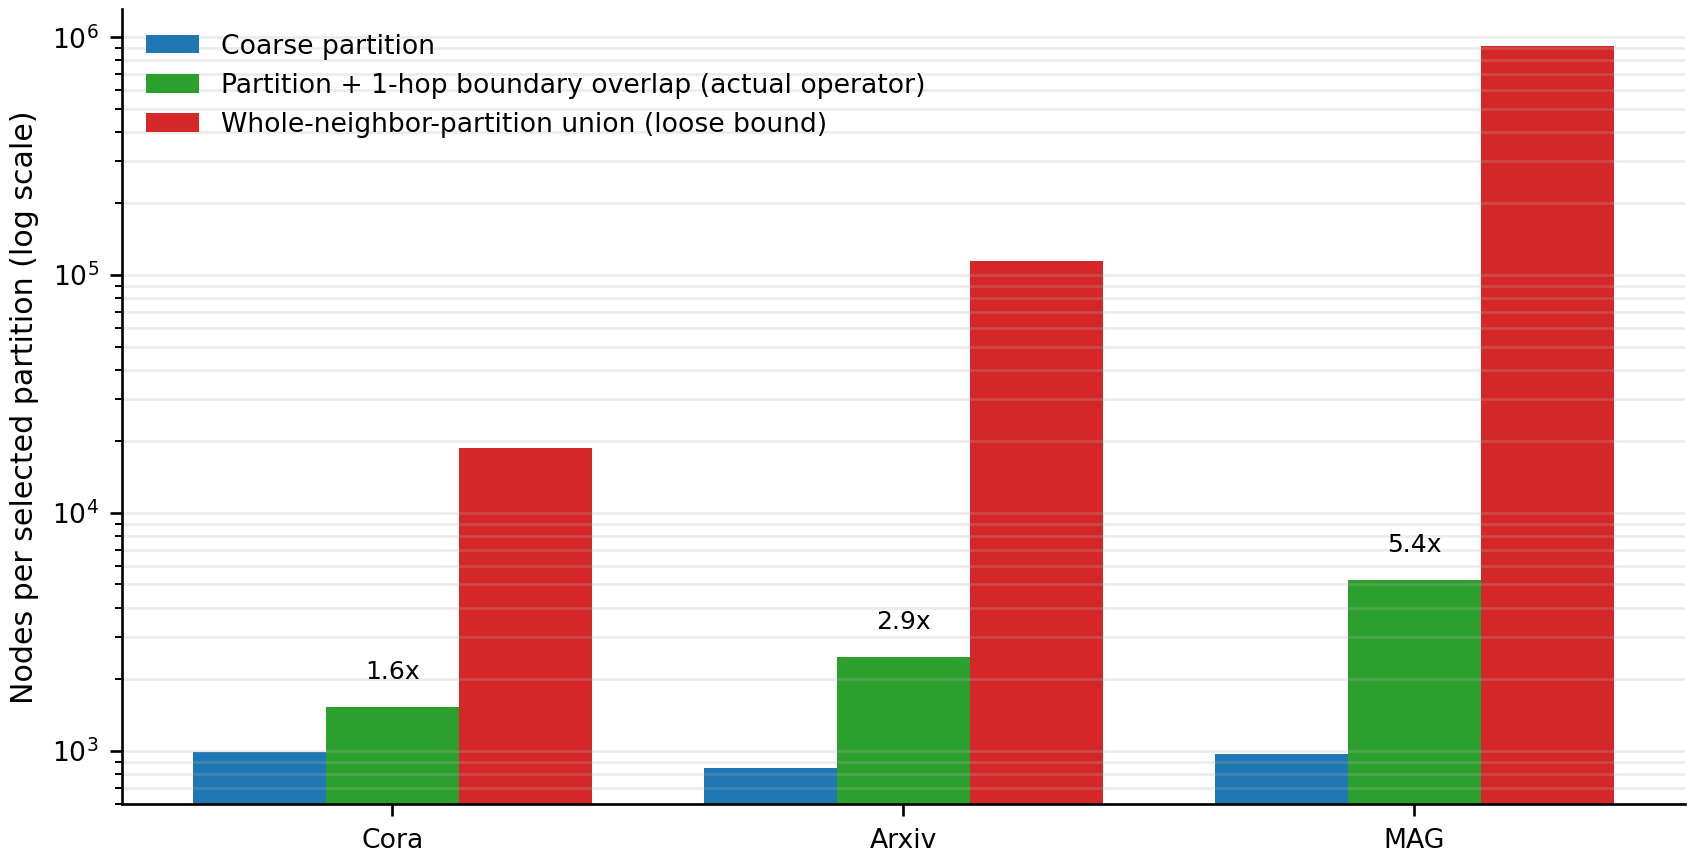
\includegraphics[width=0.92\textwidth]{fig_partition_overlap_stats.png}
\caption{\textbf{What one selected partition actually contributes (log scale).} The realized one-hop boundary overlap (green) expands a coarse partition only modestly ($1.6\times$ on Cora, $2.9\times$ on Arxiv, $5.4\times$ on MAG). The red bar is the loose union-of-whole-neighbor-partitions bound that the operator never realizes; reporting it as ``the overlap'' overstates MAG breadth by more than $170\times$. Candidate breadth instead comes from unioning these tight per-partition overlaps across the retrieval budget.}
\label{fig:partition_overlap}
\end{figure}

\section{Query-Family Breakdown and Budget Curves}
\label{app:family}

\begin{table}[h]
\centering
\caption{\textbf{Jigsaw query-family breakdown.} Positive columns report exact-solve rate; negative columns report correct no-match rate. All three datasets use the corrected connected multi-family reruns. All datasets are reported at the matched half-partition budget ($K{=}10/100/1000$); the MAG rows use the deployed MAG encoder (overall $88.6\%$).}
\label{tab:jigsaw_family}
\scriptsize
\setlength{\tabcolsep}{3pt}
\resizebox{\textwidth}{!}{%
\begin{tabular}{lrrrrrrrr}
\toprule
\textbf{Dataset} & \textbf{Single} & \textbf{K-hop} & \textbf{Deg-K} & \textbf{Walk} & \textbf{Multi-fine} & \textbf{Multi-coarse} & \textbf{Neg-label} & \textbf{Neg-struct} \\
\midrule
Cora & 100.0 & 98.3 & 97.3 & 75.3 & 100.0 & 94.3 & 100.0 & 100.0 \\
Arxiv & 100.0 & 97.3 & 98.3 & 82.3 & 100.0 & 78.7 & 100.0 & 100.0 \\
MAG & 98.7 & 93.3 & 92.7 & 71.0 & 100.0 & 76.0 & 100.0 & 99.0 \\
\bottomrule
\end{tabular}}
\end{table}

The query-family view explains the aggregate rates. At the matched half-partition budget the \emph{same} family pattern holds across all three datasets: single and multi-fine saturate, local K-hop families remain high but not perfect on MAG (K-hop $93.3\%$, degree K-hop $92.7\%$), and random-walk and multi-coarse are hardest everywhere (random-walk $75.3/82.3/71.0\%$, multi-coarse $94.3/78.7/76.0\%$ on Cora/Arxiv/MAG). These hard families arise from the query type rather than graph scale. MAG preserves high single (98.7\%) and local K-hop recovery, and its multi-region families also solve well (multi-fine 100\%, multi-coarse 76.0\%); the one family that stays hardest is random walks (71.0\%).

Random-walk queries provide the clearest stress test. FilterAll solves them at 96.0\%, and 96.6\% of Jigsaw's random-walk misses occur before Glasgow because the planted match never enters the candidate. Partition count alone does not explain this; random walks span about as many coarse partitions as K-hop queries (median 29 vs.\ 23). The difference is overlap recovery. A K-hop query forms a compact BFS ball, so nodes in a missed partition often lie on the boundary of a retrieved one and one-hop overlap recovers them 94\% of the time. A random walk is a diffuse path whose missed mid-path partitions are less often adjacent to a retrieved boundary, so overlap recovers 62\% of misses. Recovery changes from $0.94$ at size 20 to $0.40$ at size 100. The effect is milder on the smaller, denser Arxiv, where random-walk recovery is $82.3\%$ at the half-partition budget and reaches $100\%$ at all 200 partitions. On MAG, the learned retriever leads Mean-RRF by 10 points for this family and by 15 points at size 100, showing that better ranking is the effective lever once overlap cannot bridge the footprint.

MAG's high-degree quotient graph explains why ranking is the decisive mechanism. A coarse partition borders a median 948 of 2{,}000 others, and a fine partition borders a mean 568 of 10{,}000, so broad neighborhood expansion cannot selectively recover a missed mid-walk region. The inference-time probes in Appendix~\ref{app:probes} reinforce this diagnosis and identify footprint-aware representation learning as the next target. The deployed MAG encoder addresses the regime during training with a random-walk- and multi-coarse-weighted distribution of 50 to 100-node queries. Its training stream (seed 7203) is disjoint from held-out evaluation seeds 20260607/08, and the family-weighted recipe and best-FullCov checkpoint were fixed using validation seeds 31415/27182---also disjoint from the benchmark---so no benchmark query or solve rate influenced training, weighting, or checkpoint selection. Relative to a baseline encoder trained on a uniform query mix ($86.0\%$ overall, random-walk $60.0\%$, multi-coarse $71.7\%$), this targeted training lifts random-walk to $71.0\%$ and multi-coarse to $76.0\%$. Overall MAG recovery reaches \textbf{88.6\%} while preserving the easy-family results. Across all 1800 positives, the deployed Jigsaw retriever beats Mean-RRF $92$ to $35$ (exact $p{=}4.4{\times}10^{-7}$); the advantage is concentrated in multi-coarse ($34/12$) and random-walk ($44/13$), while the remaining families are statistically tied ($14/10$).

The released cumulative solved-by-budget summaries make the budget dependence explicit. With the overlap-aware retrievers, Jigsaw's cumulative solve rises $64.0/82.7/94.2/100$ on Cora (budgets 2/5/10/20), $69.6/81.3/92.8/100$ on Arxiv (20/50/100/200), and $37.6/46.0/53.0/61.9/75.4/88.6$ on MAG (20/50/100/200/500/1000) with the deployed MAG encoder; read at the half-partition budget Jigsaw solves $94.2/92.8/88.6$ on Cora/Arxiv/MAG. The $100\%$ Cora/Arxiv figures require every partition and are the exhaustive ceiling. MAG's per-size slices at $K{=}1000$ are 93.2/90.7/82.0 for sizes 20/50/100.

\begin{figure}[h]
\centering
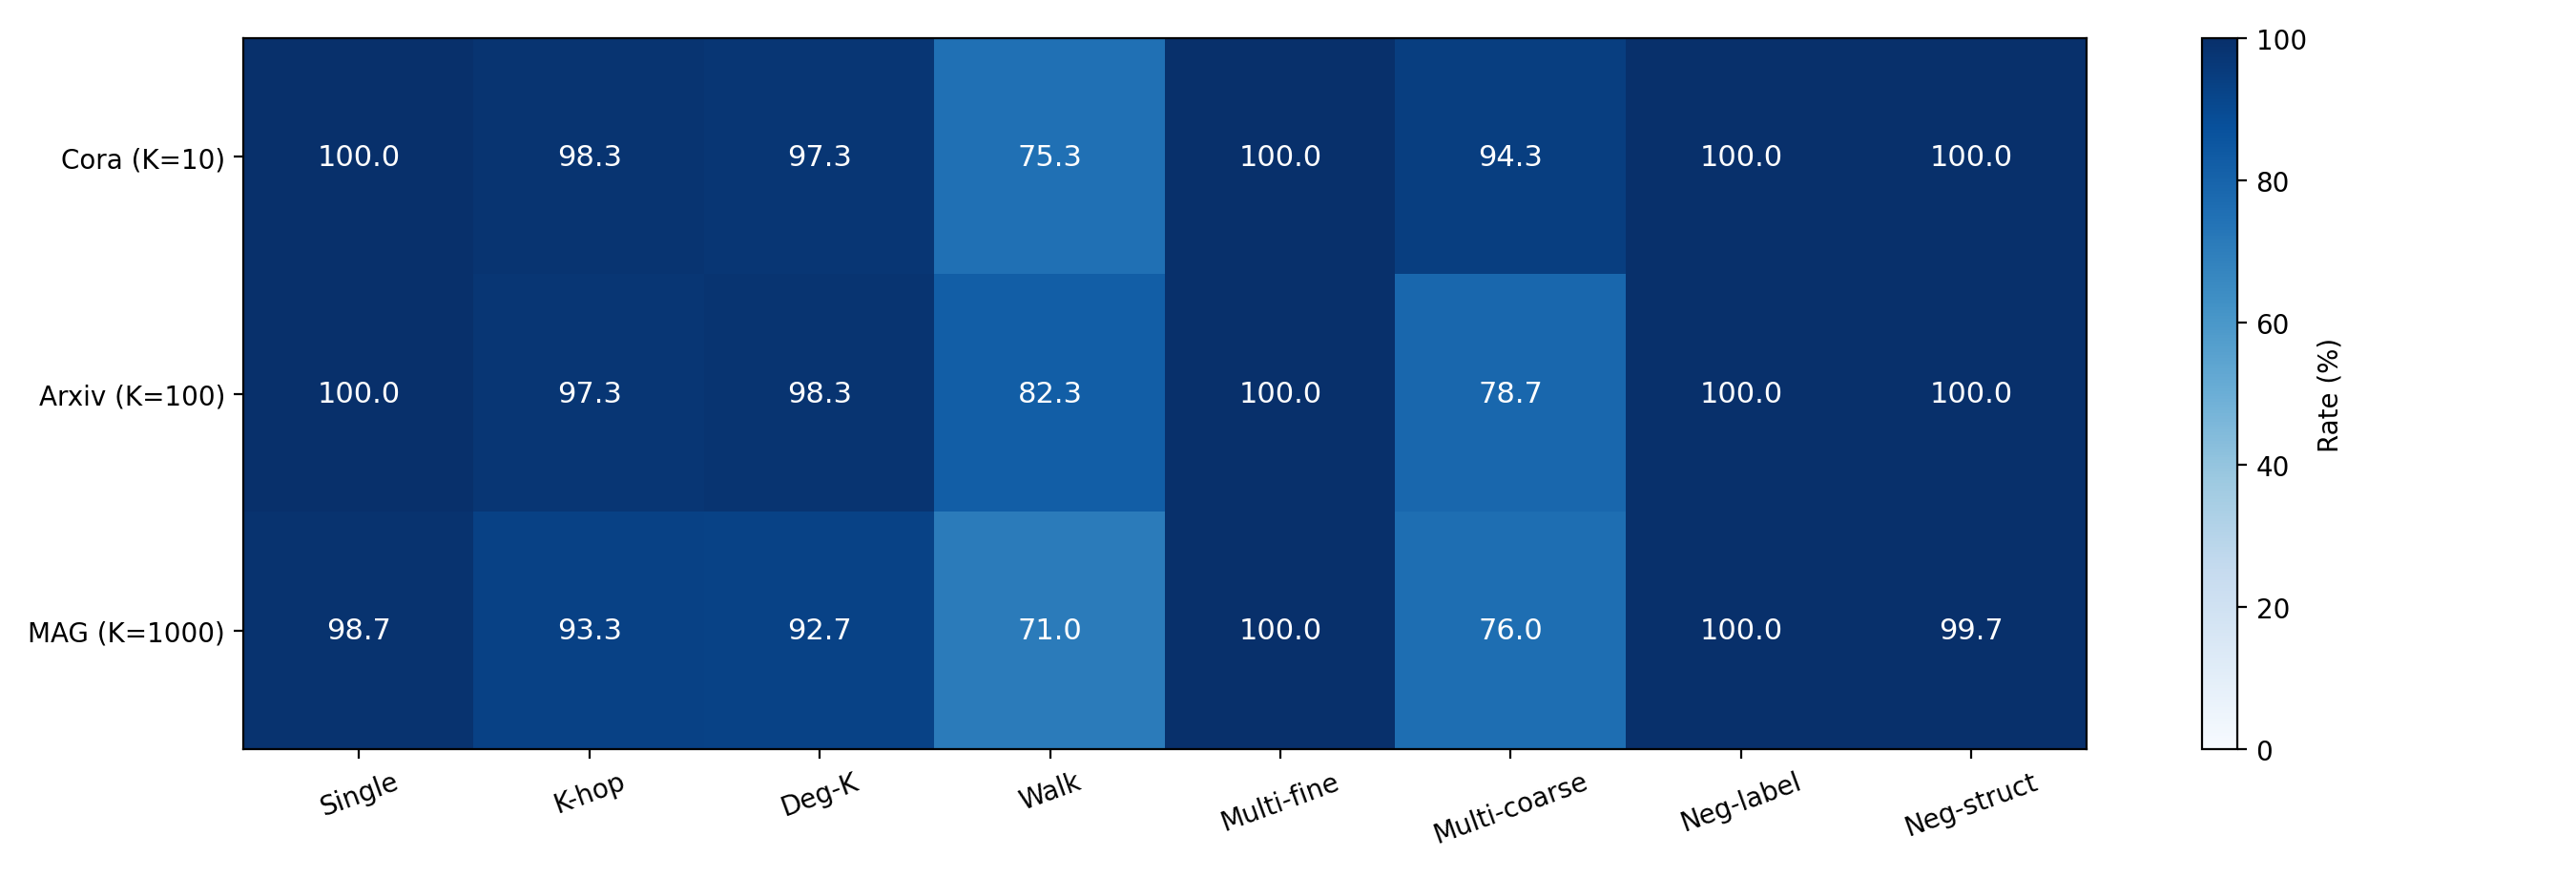
\includegraphics[width=\textwidth]{fig_jigsaw_query_family_heatmap.png}
\caption{\textbf{Jigsaw query-family outcomes.} Positive families report exact-solve rate; negative families report correct no-match rate. All rows are at the matched half-partition budget ($K{=}10/100/1000$). Random-walk and multi-coarse are the hard families across \emph{all three} datasets (Walk $75/82/71\%$, Multi-coarse $94/79/76\%$); single and multi-fine templates saturate, while local K-hop variants remain high but not perfect on MAG.}
\label{fig:query_family_heatmap}
\end{figure}

\begin{figure}[h]
\centering
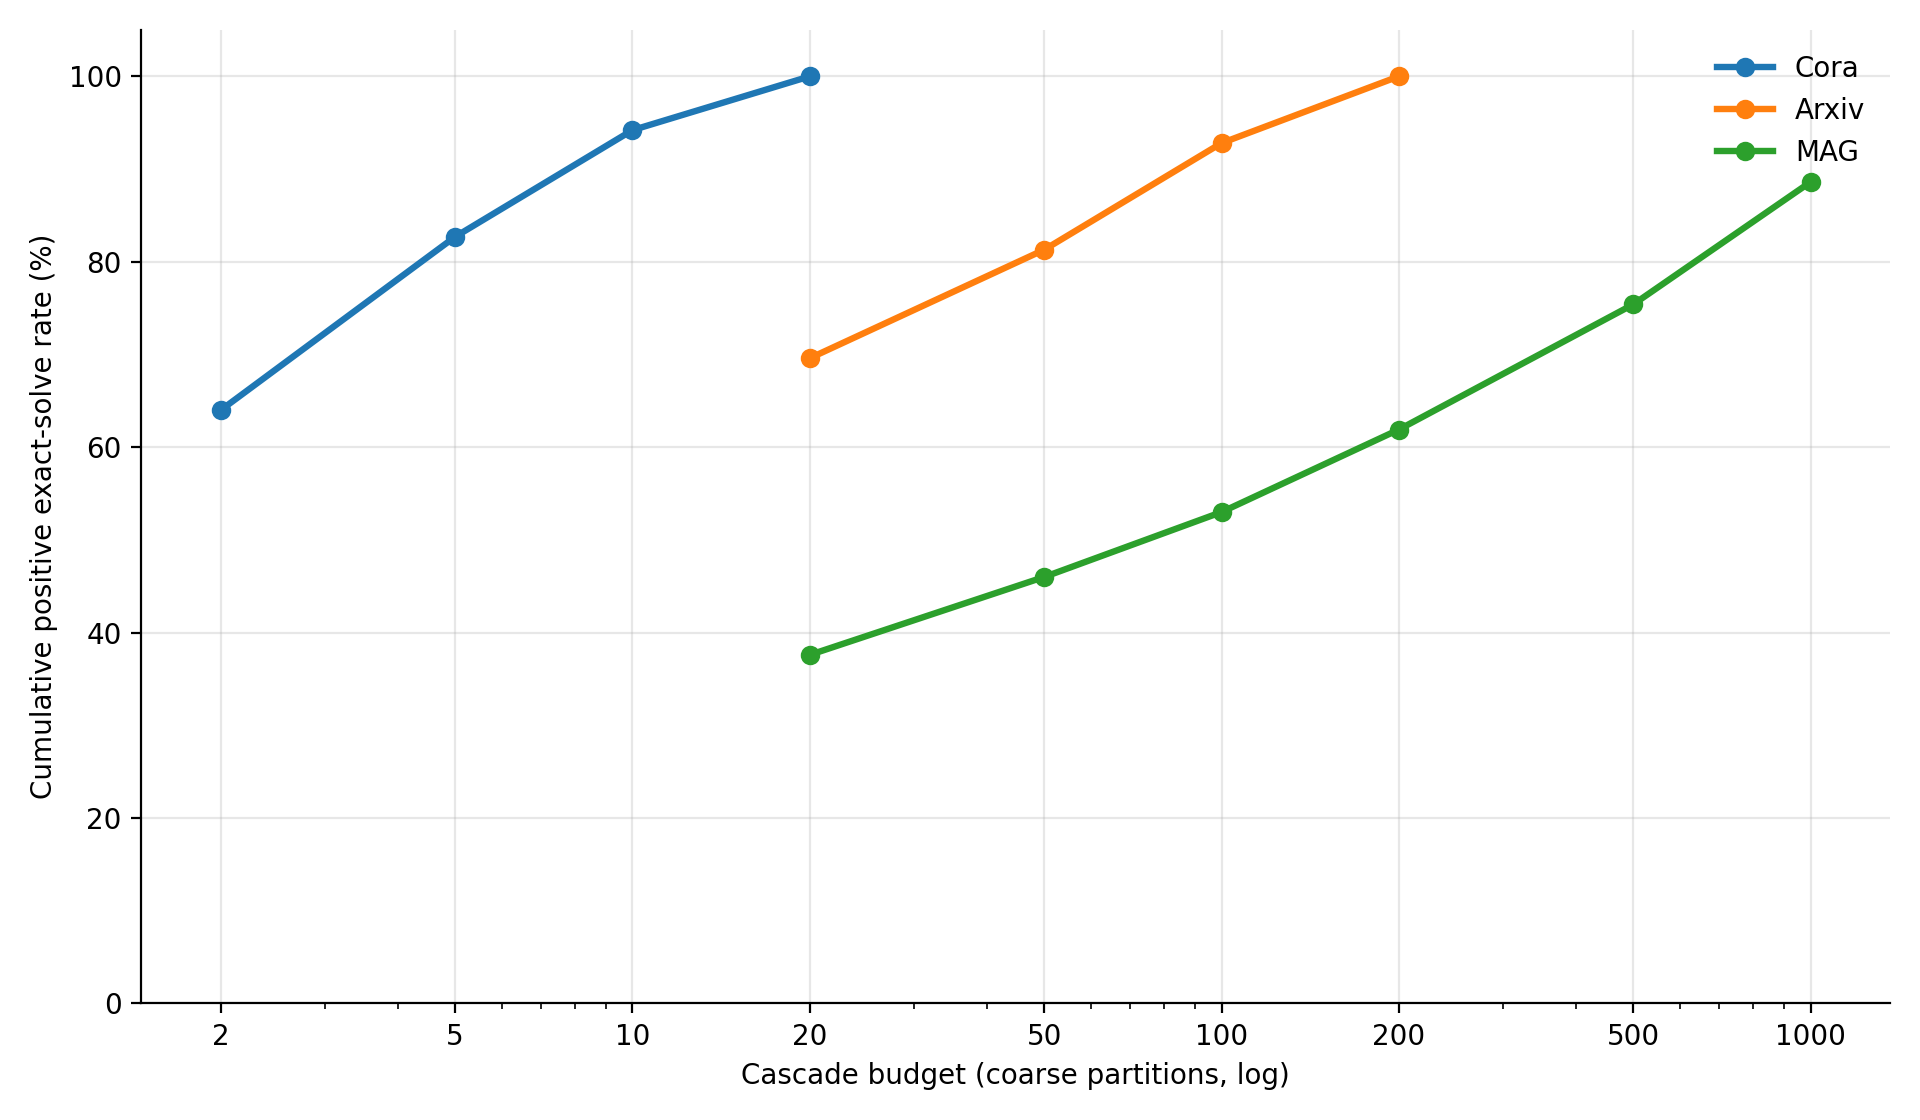
\includegraphics[width=0.92\textwidth]{fig_jigsaw_budget_curves.png}
\caption{\textbf{Solved-by-budget curves for Jigsaw.} Cora solves early because its candidate graphs are small and labels are strong. Arxiv benefits from budget expansion through 200. MAG continues improving through 1000, reflecting larger candidate regions and harder coverage.}
\label{fig:budget_curves}
\end{figure}

On Cora the curve rises steeply ($64.0\%$ at budget 2 to $100\%$ by budget 20), so a handful of partitions decides most queries. Arxiv needs budget expansion to 200 before reaching its final positive solve rate, even though all policies eventually reach 100\%. MAG continues to improve through 500 and 1000, which means failures at small budgets are often not verifier unsoundness but insufficient candidate expansion. This supports exposing budget as a control knob rather than using one fixed candidate size for all queries.

\clearpage
\begin{figure}[H]
\centering
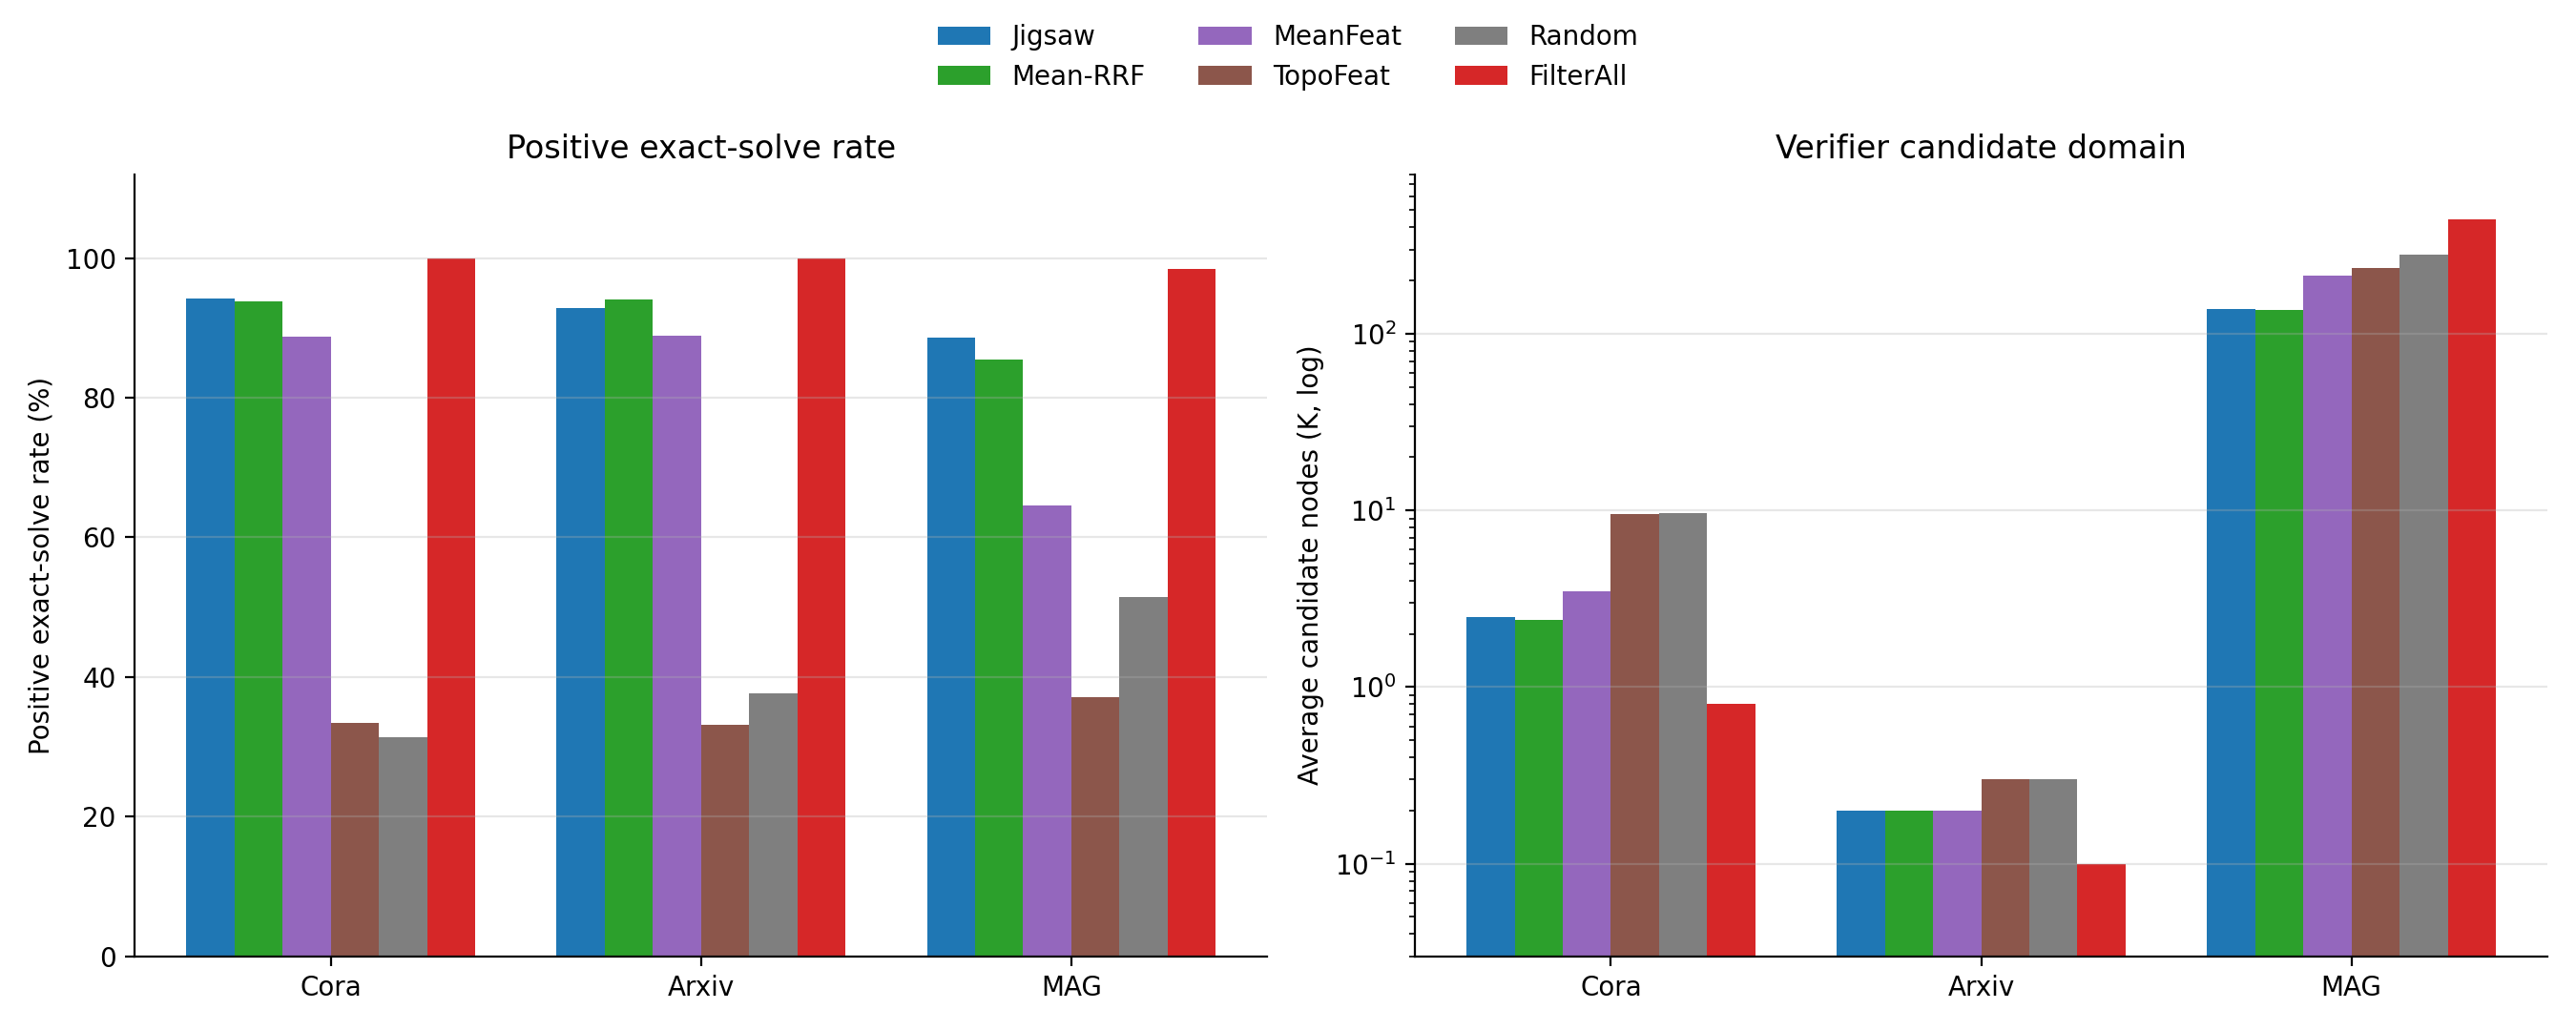
\includegraphics[width=\textwidth]{fig_production_positive_rates.png}
\caption{\textbf{Main-benchmark positive solve rates and cost.} Left: positive exact-solve rate at half-partition budgets ($K{=}10/100/1000$); FilterAll is the exhaustive ceiling. Right: mean pruned candidate nodes at those same endpoints (FilterAll at the all-partition ceiling).}
\label{fig:production_rates}
\end{figure}

\section{Expanded MAG Results and Statistical Significance}
\label{app:mag_narrative}

This appendix gives the per-family, cost, and significance details behind the condensed MAG discussion and Table~\ref{tab:production_matrix}. The reported aggregates are the same as those in the body.

\paragraph{Matched Cora/Arxiv cost and difficulty.} At the same half-partition endpoints used for solve rate, Jigsaw sends a mean 458/77 terminal candidate nodes on Cora/Arxiv and completes the cascade in 0.05/0.19\,s (11.8/18.3\,ms in the verifier). Cora size-100 recovery is lower and costlier than sizes 20/50 ($89.0\%$ vs. $96.8/96.8\%$; 0.071\,s vs. 0.036/0.047\,s), driven by random-walk ($75.3\%$). Arxiv similarly declines to $90.3\%$ at size 100 from $93.8/94.2\%$, with multi-coarse hardest ($78.7\%$); single and multi-fine remain $100\%$ on both graphs. FilterAll selects every partition, but exact-label pruning reduces its terminal verifier domain to only 59/57 nodes. Its exhaustive cost comes from retrieval scope and residence, not a large post-pruning graph.

\paragraph{The MAG lower bound and scaling crossover, in full.} Direct Glasgow solves 0/15 full-MAG K-hop queries and 0/15 on Arxiv, versus 15/15 on Cora. On those same Cora/Arxiv queries, Jigsaw at matched half-partition budgets solves 15/15 in median $0.03/0.11$\,s with about 50 pruned nodes. The Cora cascade result therefore does not rely on retrieving all 20 partitions. FeatureIndex is strongest under near-unique MAG labels, FilterAll is the recall ceiling, and learned retrieval is useful under bounded memory and coarse labels. On MAG, Jigsaw uses fewer candidate nodes than FilterAll (138K versus 444K) and lower verifier time (82 ms versus 289 ms), although candidate construction remains the dominant cost.

\paragraph{Statistical significance.}
Bootstrap 95\% confidence intervals on the MAG positive solve rate (n${=}1800$ queries per method) and paired exact-McNemar tests (pairing per query so wins/losses count only queries two policies decide differently) confirm the ordering. Among the retrieval \emph{components}, the FullCov-trained retriever significantly outperforms the other learned and feature retrievers (Mean-RRF, re-evaluated under the same deployed encoder, 92 vs 35 wins, $p{=}4.4{\times}10^{-7}$; mean features / random / topology $p<10^{-76}$), and FilterAll significantly exceeds it (225 vs 2 wins, $p{=}2.4{\times}10^{-64}$) as the exhaustive ceiling; the latter four are encoder-independent and reported against the baseline-encoder Jigsaw. These comparisons evaluate retrieval components within the same system. The paper's contribution is exact matching at million-node scale without holding the graph resident. The retriever keeps the candidate both small and memory-bounded, sending the verifier $3.2\times$ fewer candidate nodes than the exhaustive FilterAll ceiling, and FullCov improves coverage on the hard families relative to the matched learned/fusion baselines.

\paragraph{Candidate construction is volume-bound.} Mean per-query candidate-build time is 3.4\,s for Jigsaw and 5.5\,s for FilterAll, compared with 0.25\,s for exact solving (Section~\ref{sec:shrinkage}, fact 3). These means come from the baseline-encoder shrinkage run. The main-benchmark cascade times use the deployed encoder and also exclude retrieval/ranking, but the two runs are not directly additive. Node volume, not the union implementation, sets the build cost: a verified-equivalent vectorized tensor union runs between $0.5$ and $0.9\times$ as fast as the set union. The practical latency lever is therefore better localization, which reduces the number of boundary nodes admitted before exact verification.

\begin{figure}[H]
\centering
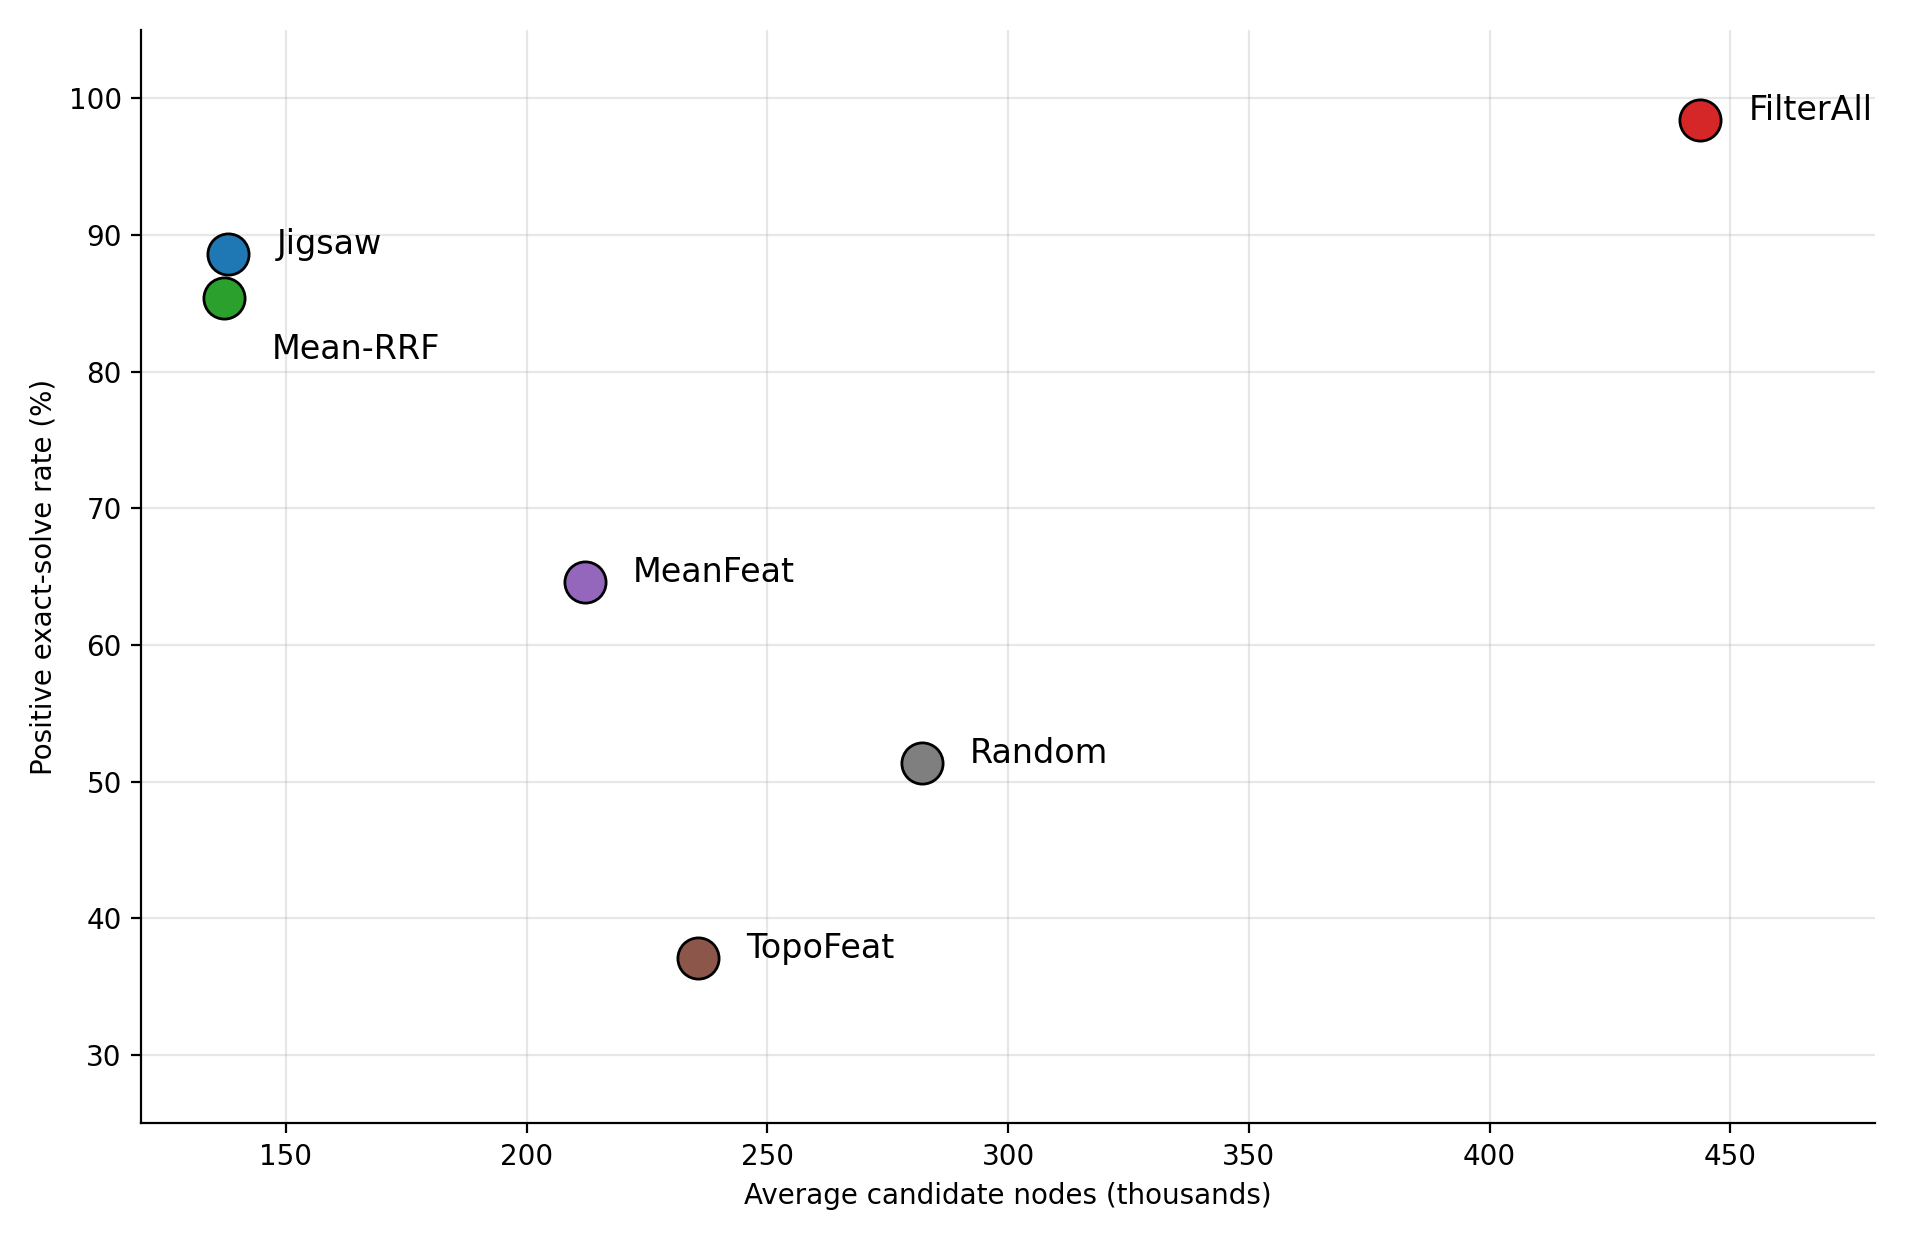
\includegraphics[width=\textwidth]{fig_mag_tradeoff.png}
\caption{\textbf{MAG tradeoff.} MAG is the realistic large-scale dataset where retrieval policies separate sharply. FeatureIndex is strongest under near-unique labels; FilterAll is the exhaustive ceiling; learned Jigsaw is a memory-bounded operating point that uses less than half the candidate nodes of FilterAll.}
\label{fig:mag_tradeoff}
\end{figure}

\begin{figure}[H]
\centering
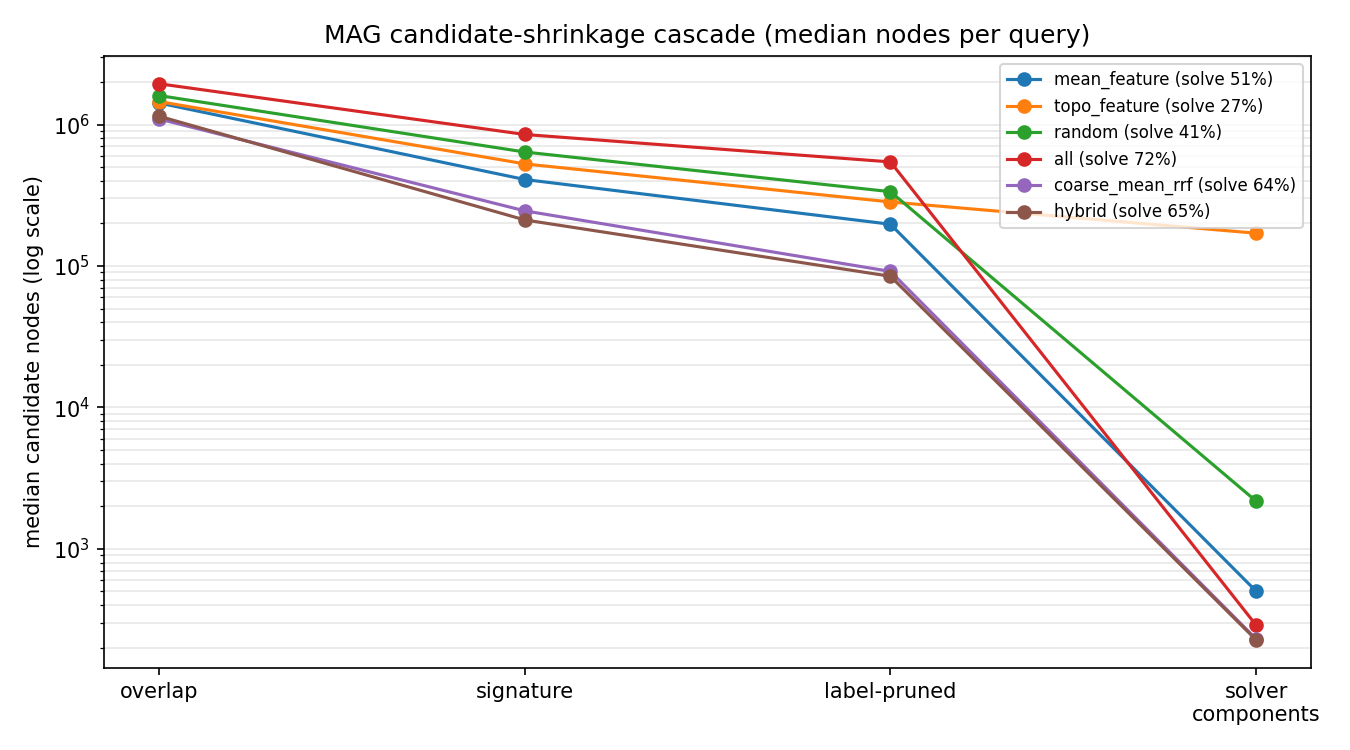
\includegraphics[width=0.95\textwidth]{fig_candidate_shrinkage_mag.png}
\caption{\textbf{MAG candidate-shrinkage cascade (median nodes per query, log scale).} Each policy's candidate is tracked through overlap, signature, label pruning, and component decomposition. Learned retrieval (Jigsaw) and Mean-RRF reach much smaller solver inputs than uninformed policies, and far smaller than FilterAll, even though all share the same lossless pruning.}
\label{fig:shrinkage}
\end{figure}

\begin{samepage}
\section{System-Design Ablations and Model-Variant Diagnostics}
\label{app:design}

The operators remain dataset-dependent, but the equal-budget comparison removes the full-budget confound. On MAG, removing one-hop overlap halves solve rate ($88.9{\to}44.4\%$), while signatures are inert ($88.9\%$ and about $151$K candidates with or without them). On Arxiv, overlap has a smaller but real effect ($94.4{\to}86.1\%$). Signatures are the main candidate-control mechanism there, expanding the mean pruned domain ${\sim}37\times$ ($76{\to}2{,}815$) when removed. Exact-label pruning reduces Arxiv candidates ($244{\to}76$) and remains important for negatives; removing it lowers MAG solve rate ($88.9{\to}52.8\%$). Component decomposition also helps MAG ($88.9{\to}63.9\%$ without it). Together with the Arxiv retrieval ablation in Table~\ref{tab:loss_ablation}, these results separate the learning gain from the execution gains supplied by overlap, pruning, and component solving.
\end{samepage}

\begin{table}[H]
\centering
\caption{\textbf{Operator-necessity ablation at matched half-partition budgets.} The shared diagnostic has 48 queries per dataset; solve and candidate statistics use its 36 planted positives. We report MAG at $K=1{,}000/2{,}000$ and Arxiv at $K=100/200$. Candidate count is the mean pruned domain at the first solved budget at or below $K$, or the largest attempted budget at or below $K$ when unsolved.}
\label{tab:design_ablation}
\scriptsize
\setlength{\tabcolsep}{5pt}
\resizebox{\textwidth}{!}{%
\begin{tabular}{lrrrr}
\toprule
 & \multicolumn{2}{c}{\textbf{OGBN-MAG}} & \multicolumn{2}{c}{\textbf{OGBN-Arxiv}} \\
\cmidrule(lr){2-3}\cmidrule(lr){4-5}
\textbf{Variant} & \textbf{Solve \%} & \textbf{Cand.} & \textbf{Solve \%} & \textbf{Cand.} \\
\midrule
Full Jigsaw    & 88.9          & 150.6K & 94.4 & 76 \\
No overlap     & \textbf{44.4} & 152.5K & \textbf{86.1} & 88 \\
No signature   & 88.9          & 150.7K & 94.4 & \textbf{2{,}815} \\
No components  & 63.9          & 143.0K & 94.4 & 76 \\
No exact-label & 52.8          & 223.6K & 94.4 & 244 \\
\bottomrule
\end{tabular}}
\end{table}

\begin{figure}[H]
\centering
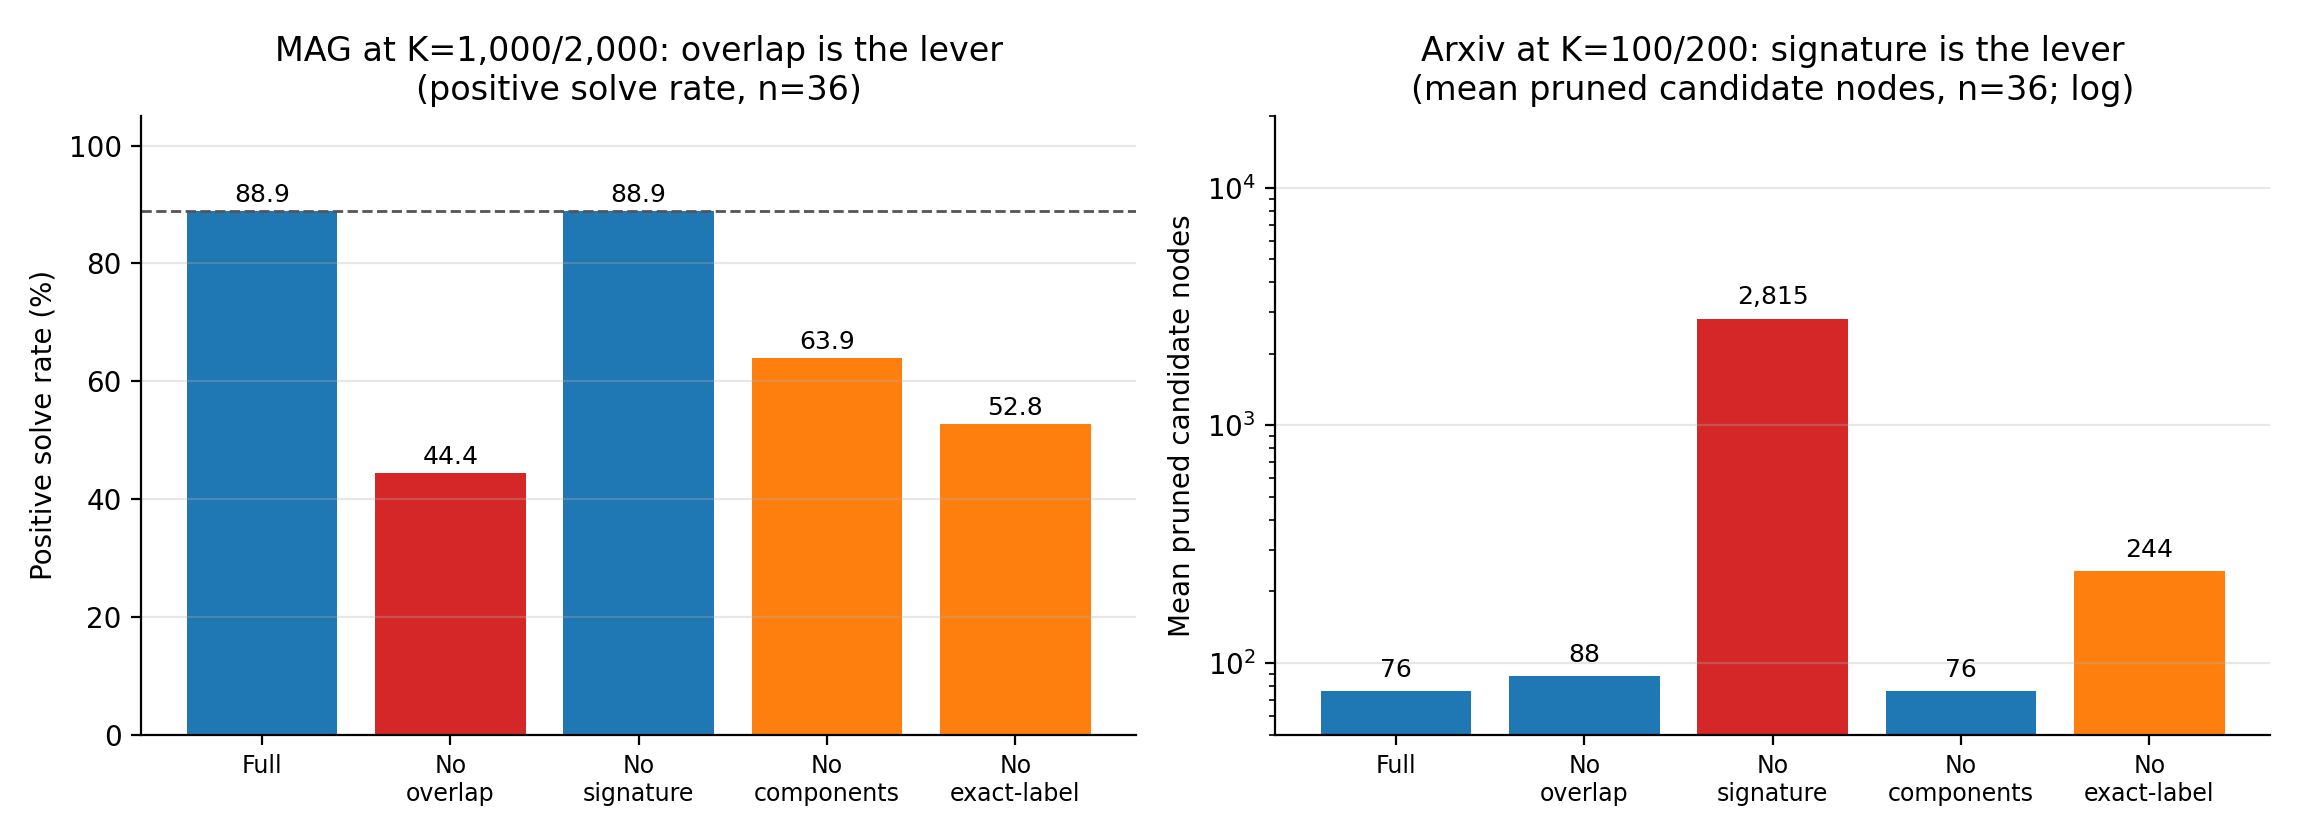
\includegraphics[width=0.92\textwidth]{fig_design_ablation.png}
\caption{\textbf{Operator necessity at matched half-partition budgets.} \emph{Left:} on MAG, disabling overlap halves solve rate ($88.9{\to}44.4\%$). \emph{Right:} on Arxiv, disabling signatures expands mean pruned candidates ${\sim}37\times$ ($76{\to}2{,}815$, log axis); removing overlap lowers solve rate ($94.4{\to}86.1\%$).}
\label{fig:design_ablation}
\end{figure}

\paragraph{Model-variant diagnostics.}
We retain model-variant diagnostics outside the main benchmark. On Arxiv, extended training changes retrieval behavior, but the reported result uses the checkpoint selected before evaluation in a balanced two-seed matrix. On MAG, we evaluated both the validation-selected and final-epoch checkpoints. The main result uses the former because validation FullCov selected it; the latter is reported separately and is not averaged into the benchmark.

\section{Retrieval Remedies and Cross-Dataset Selectivity}
\label{app:probes}

\paragraph{The label-selectivity crossover generalizes.} Repeating the retrieval comparison on Cora and OGBN-Arxiv (retrieval-only, identical query families, $n{=}540$ each) reproduces the MAG inversion (Table~\ref{tab:selectivity_xd_log}). It tracks the median number of partitions spanned by a label, an offline statistic (Cora feature labels $1$, class $12$; Arxiv feature $1$, class $124.5$). Under near-unique feature labels the classical index ties the learned retriever on contained families and wins overall (Cora rank $2$ vs.\ $5$; Arxiv $4$ vs.\ $44$); under realistic class labels it collapses toward random (Arxiv $104$ of $200$) while the learned retriever wins every family (Cora $5$ vs.\ $7$; Arxiv $44$ vs.\ $104$; per-query sign test $p<10^{-30}$ in both regimes, $n{=}540$). Selecting the retriever by this offline signal is a deployable, non-oracle portfolio; on Cora/Arxiv it is a localization (retrieval-rank) result, corroborated end-to-end only on MAG.

\begin{table}[H]
\centering
\caption{Cross-dataset label-selectivity crossover: overall median worst-true-partition rank (lower is better; retrieval-only, $n{=}540$ per dataset = 2 seeds $\times$ 6 positive families $\times$ 3 sizes $\times$ 15 queries).}
\label{tab:selectivity_xd_log}
\small
\begin{tabular}{lcccc}
\toprule
 & \multicolumn{2}{c}{FeatureIndex} & Learned & Parts/label \\
\cmidrule(lr){2-3}
Dataset (parts) & feature & class & (any) & feat / class \\
\midrule
Cora ($20$)   & 2 & 7   & 5  & $1$ / $12$ \\
Arxiv ($200$) & 4 & 104 & 44 & $1$ / $124.5$ \\
\bottomrule
\end{tabular}
\end{table}

\paragraph{The crossover also appears within MAG as label selectivity falls.} Holding the 1.9M-node target fixed and shrinking the md5 codebook from $10^6$ to $10^2$ distinct labels drives the median partitions spanned by a label from $1$ to $1{,}938$ (Table~\ref{tab:mag_selectivity_sweep}). The learned ranker never uses this codebook, so its coverage is a single value per family, invariant to the sweep; only FeatureIndex moves. On the three feature-driven families FeatureIndex begins at the ceiling under near-unique labels and falls monotonically as selectivity drops, crossing below the learned ranker family by family: multi-coarse once labels span a few hundred partitions, and the near-templated single/multi-fine families only past ${\sim}1{,}900$. This reproduces the cross-dataset inversion of Table~\ref{tab:selectivity_xd_log} on a single deployed target, so the learned advantage is a low-selectivity phenomenon rather than a dataset artifact. The spatially diffuse families are governed by footprint, not label selectivity, and are analyzed separately below.

\begin{table}[H]
\centering
\caption{\textbf{Within-MAG label-selectivity sweep} (FullCov@$1000$, feature-driven families, $n{=}300$ each). As the md5 codebook shrinks, the median partitions spanned by a label grows and FeatureIndex coverage falls monotonically, crossing below the \emph{label-independent} learned ranker (bottom row, flat by construction). Multi-coarse is overtaken first; the near-templated single/multi-fine families resist until labels span ${\sim}1{,}900$ partitions.}
\label{tab:mag_selectivity_sweep}
\small
\setlength{\tabcolsep}{6pt}
\begin{tabular}{lrrr}
\toprule
Median parts/label & Single & Multi-fine & Multi-coarse \\
\midrule
$1$ (near-unique)   & 100.0 & 100.0 & 99.0 \\
$7$                 & 100.0 & 100.0 & 99.0 \\
$74$                & 100.0 & 100.0 & 94.0 \\
$636$               & 100.0 & 100.0 & 59.3 \\
$1{,}938$           & 76.0  & 78.7  & 14.0 \\
\midrule
Learned (flat)      & \textbf{99.3} & \textbf{99.7} & \textbf{65.0} \\
\bottomrule
\end{tabular}
\end{table}

\paragraph{Spatially extended queries require representation-level coverage.} On MAG, subquery multi-vector MaxSim, finer partition parents, one- and two-hop fine-level overlap, dual-granularity late interaction, and coarse diffusion all leave FullCov@1000 within ${\approx}2$ points of the single-vector baseline on the k-hop/degree-k-hop/random-walk families (Table~\ref{tab:probes_log}); the best gain is ${\approx}{+}2.3$ (coarse diffusion), while a coarse neighbor-stitch expansion reduces coverage by $8$ to $13$ points. The cause is density: the partition graph is high-degree at every granularity (median coarse degree $948$ of $2{,}000$; mean fine degree $568$ of $10{,}000$), so neighborhood-following broadens the candidate rather than tracing the query footprint. This evidence directs further improvement toward coverage-aware representation learning.

\begin{table}[H]
\centering
\caption{Inference-time remedies on the same 1,800-query MAG positive workload: FullCov@$1000$ (\%). Each displayed spatial family has $n{=}300$ queries.}
\label{tab:probes_log}
\small
\begin{tabular}{lrrr}
\toprule
Method & k-hop & degree-k-hop & random-walk \\
\midrule
Single-vector (current)           & 14.7 & 17.3 & 9.0 \\
Subquery MaxSim (query-only)      & 14.3 & 17.7 & 8.0 \\
Finer partition parent            & 12.7 & 16.7 & 8.3 \\
Fine-level overlap (1-hop)        & 13.3 & 17.3 & 10.0 \\
Fine-level overlap (2-hop)        & 13.3 & 18.3 & 9.3 \\
Dual-granularity late interaction & 12.7 & 16.0 & 8.7 \\
Coarse diffusion                  & 17.0 & 19.7 & 10.3 \\
\bottomrule
\end{tabular}
\end{table}

\section{Memory-Bounded Streaming Serve}
\label{app:memory}

The streaming serve holds only an LRU cache of partitions resident and fetches the rest from disk in a two-pass sweep (nodes, then edges), so peak resident memory is bounded by the cache size rather than by the graph. The conservative primary serve reported in the body uses $2.4$\,GB versus $10.2$\,GB for whole-graph residence ($4.2\times$ smaller). Figure~\ref{fig:memory_latency} additionally reports an optimized cache sweep whose eight-partition point is $1.9$\,GB. Both implementations make memory a tunable resource; their cold-load latency is competitive and load-dominated, and larger caches buy down tail latency.

\begin{figure}[H]
\centering
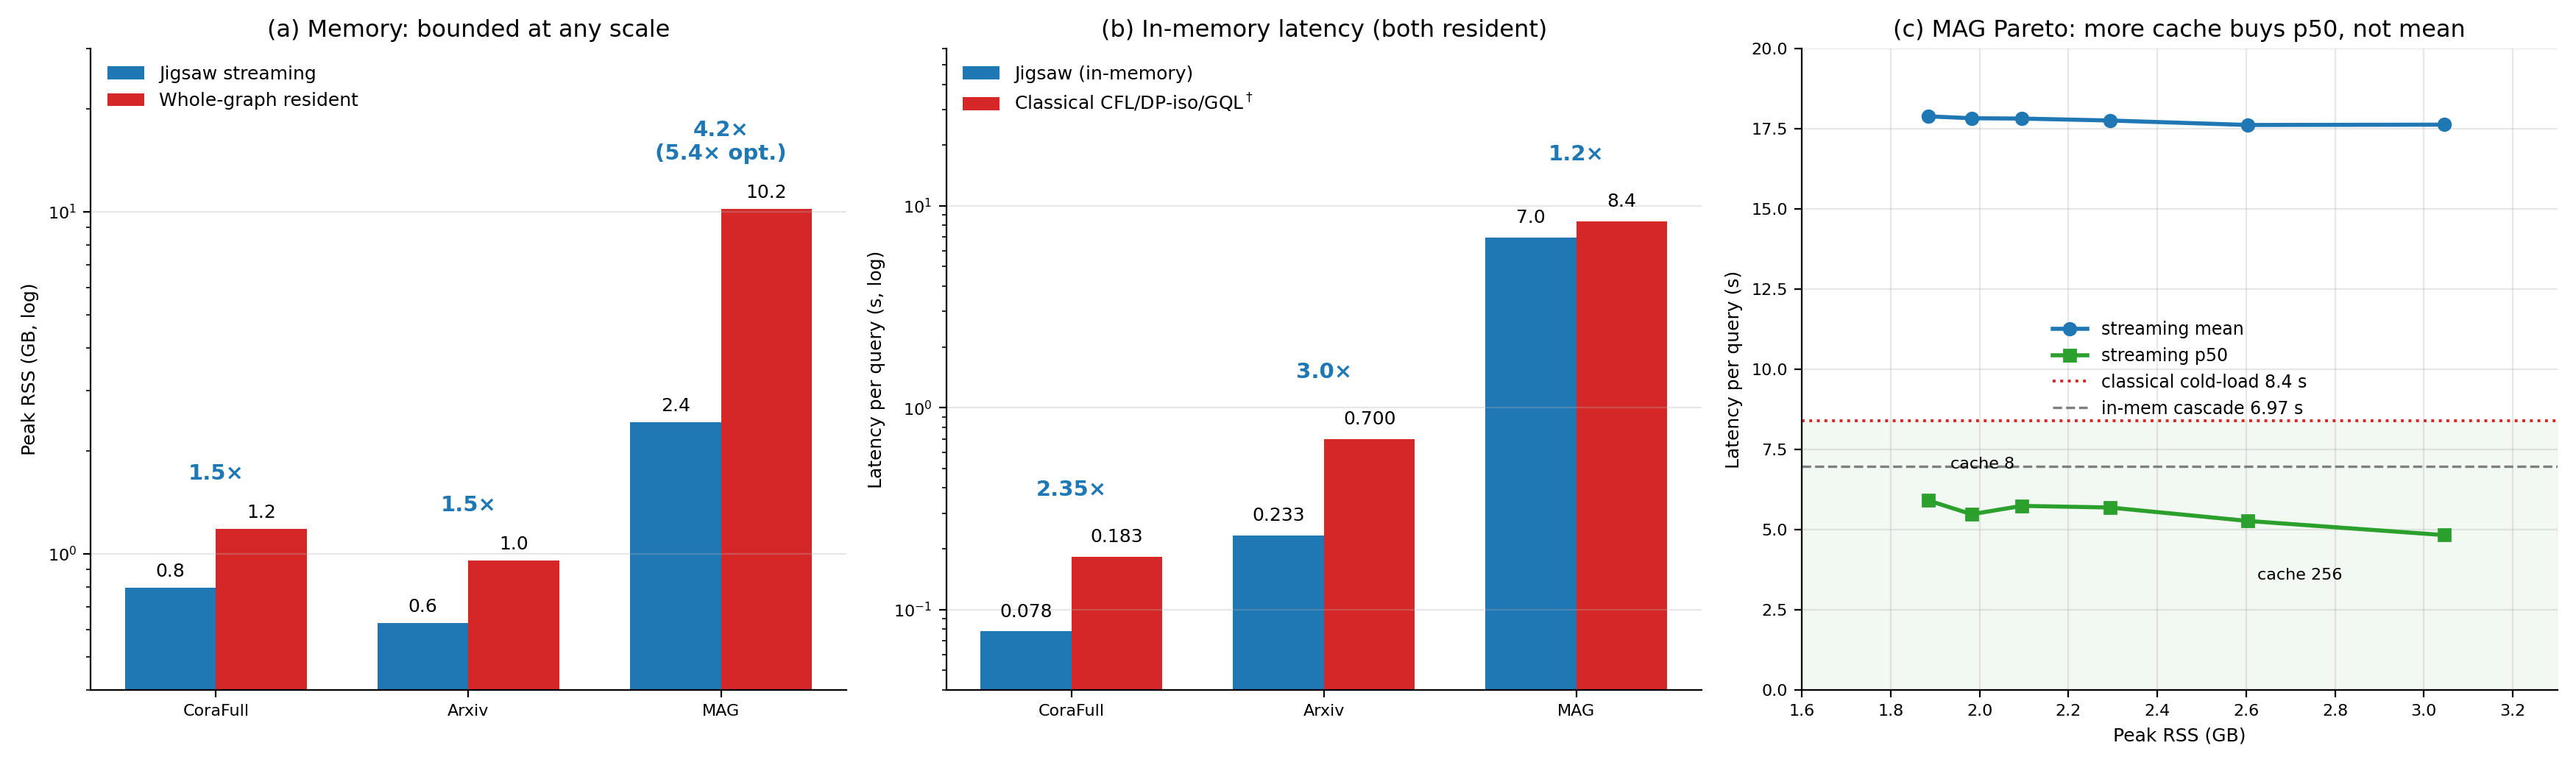
\includegraphics[width=\textwidth]{fig_memory_latency.png}
\caption{\textbf{Memory is the primary benefit; cold-load latency is competitive and the tradeoff is tunable.} \textbf{(a)} The conservative primary streaming serve is $4.2\times$ smaller on MAG ($2.4$ vs $10.2$\,GB); the optimized cache sweep shown here lowers its eight-partition point to $1.9$\,GB ($5.4\times$). \textbf{(b)} Cold-load end-to-end latency, Jigsaw vs.\ classical CFL/DP-iso/GQL: $2.35$/$3.0$/$1.2\times$ faster on Cora/Arxiv/MAG because Jigsaw avoids the full-graph load ($^\dagger$MAG resident enumeration is ${\sim}1$\,ms after loading). \textbf{(c)} MAG memory$\leftrightarrow$latency frontier as the cache grows ($8{\to}256$): more memory buys down p50 ($5.9{\to}4.8$\,s, below the $8.4$\,s cold-load) while the mean remains $17.9$ to $17.6$\,s because of a hard-query I/O tail. Jigsaw lets the operator choose a frontier point an all-or-nothing resident matcher cannot.}
\label{fig:memory_latency}
\end{figure}

\section*{GenAI Usage Statement}
Generative AI tools assisted with implementation, experiment orchestration, data-validation scripts, and manuscript language editing. The authors reviewed and verified all AI-assisted code, analyses, numerical claims, and text, and take full responsibility for the final work.

\end{document}
